\chapter{Evaluation}
\label{ch:evaluation}

We will now evaluate the benefit of the two independent optimizations we
proposed to next word prediction: representing language model probabilities as
weighted sums (\cref{ch:weightedsum}) and calculating the word with the highest
probability via top-$k$ joining (\cref{ch:topkjoin}).
To this end we empirically compare their performance in a variety of usage
scenarios.

This chapter is organized as follows:
first the experimental setup used over all experiments is described in
\cref{sec:experimental-setup}, then our form of data visualization is explained
in \cref{sec:boxplot}, and finally weighted sums are evaluated in
\cref{sec:evaluation-weightedsum} and top-$k$ joining in
\cref{sec:evaluation-topkjoin}.


% ------------------------------------------------------------------------------
\section{Experimental Setup}
\label{sec:experimental-setup}

As explained in \cref{ch:review}, the calculations of the considered language
models' probabilities depend on occurrence counts obtained through statistical
analysis of text corpora.
For this evaluation the \emph{Open American National Corpus (OANC)} by
\textcite{OANC} was used.
It is a free collection of written text and transcripts of spoken data,
featuring both historical and contemporary American English of all genres.
It contains around 600 thousand sentences which amount to 14 million words in
total.

In our experiments only the written part of that corpus was used, because next
word prediction has no application to speaking.
The corpus comes tagged with semantic sentence boundaries which were used to
split the data into sentences.
No begin or end of sentence tags were inserted, as to not falsify the actual
occurrence counts.
Tokenization was performed by assuming word boundaries to occur at each space.
To avoid punctuation marks directly following words being counted as only one
word, all special characters were surrounded by spaces.
This means for our analysis, punctuation marks count as regular words.
This has the downside of text like \texttt{you're} becoming \texttt{you ' re}.
Other than that, the data was left as is.
In particular no case normalization, stemming or removing of names was
performed.

That text was then randomly split into 80\% training and 20\% heldout data.
To measure how the algorithms under examination behaved for different sizes
of training data, we successively discarded 50\% of sentences from training.
Through this we obtained five datasets equaling 100\%/50\%/25\%/12.5\%/6.25\%
of the original training corpus size.
\Cref{tab:evaluation-trainings} shows the different datasets.
Distinct language models were then learned on each of these training sets.

\begin{table}
  \hspace{-0.35cm}
  \begin{tabular}{lrrr}
    \toprule
    Corpus & No.\ Sentences & No.\ Unique Words & Raw File Size \\
    \midrule
    \texttt{OANC}            & \num{608277} & \num{196345} & \SI{71.0}{\mebi\byte} \\
    \texttt{Training-100\%}  & \num{486409} & \num{178671} & \SI{57.0}{\mebi\byte} \\
    \texttt{Training-50\%}   & \num{243204} & \num{133038} & \SI{29.0}{\mebi\byte} \\
    \texttt{Training-25\%}   & \num{121602} & \num{ 98209} & \SI{15.0}{\mebi\byte} \\
    \texttt{Training-12.5\%} & \num{ 60801} & \num{ 70988} & \SI{ 7.1}{\mebi\byte} \\
    \texttt{Training-6.25\%} & \num{ 30400} & \num{ 50372} & \SI{ 3.6}{\mebi\byte} \\
    \bottomrule
  \end{tabular}
  \caption{Overview of the different datasets used for training.}
  \label{tab:evaluation-trainings}
\end{table}

From the heldout data \num{40000} non-overlapping sequences of ten words were
selected.
For our experiments all but the last words of that sequence were considered to
form the history, and the last word then is the word for which either a
probability is calculated, or which is expected to be predicted by next word prediction.
For cases were shorter histories of words were needed, words were removed from
the front of the sequences, so the words whose probability are calculated
respectively which are predicted remain the same.
To avoid the problem of how to handle unknown words in the evaluation, these
sequences were chosen as to not contain any words, that do not occur in
the smallest 6.25\% training corpus.
Because of this no pruning of words had to be performed, and an \texttt{UNK}
token was not assigned an artificially occurrence count.

The evaluation was performed using the \emph{Generalized Language Modeling
Toolkit (GLMTK)}\footnote{The \emph{Generalized Language Modeling Toolkit
(GLMTK)} is freely available under
\mbox{\url{https://github.com/renepickhardt/generalized-language-modeling-toolkit/}}.},
a freely available toolkit in Java to compare different language modeling
techniques, that I wrote as part of my work as a student research assistant.
Initially it was able to perform the traditional, recursive calculations for
both Modified Kneser-Ney Smoothing and the Generalized Language Model.
For this thesis I implemented next word prediction using all optimizations
described in \cref{ch:weightedsum,ch:topkjoin} as well as all experiments from
this chapter.
\todo{Tag bachelor commit and mention in footnote.}

All experiments were run on a virtual machine that was assigned eight
\SI{3.0}{\giga\hertz} processor cores, each with a cache size of
\SI{4096}{\kibi\byte}.
Although multiple cores were available, all experiments were run in a single
thread, one after another, to avoid thread communication influencing the
benchmark.
We used Linux (3.2.0-75-virtual) as the operating system, and
the OpenJDK with java version 1.7.0\_79 as the implementation of the
Java Platform.
The Java Virtual Machine (JVM) was assigned \SI{16}{\gibi\byte} of main memory,
a limit that none of the experiments hit.

Java Virtual Machines are know to exhibit \enquote{warm-up} behavior \noref.
That is it takes some time while running a program to find hotspot sections
in the code and JIT compile these.
Traditionally experimenters want to avoid that benchmarks are distorted by
this warm-up behavior \noref.
To circumvent this, the code under benchmark is usually executed multiple times,
to ensure JIT compilation of the relevant sections, and the actual benchmark
is only performed afterwards.
To this end, we decided to run each experiment twice:
the first execution is for warming-up the Java Virtual Machine, while actual
tracking of performance metrics only occurs in the second run.
As each experiment consists of executing \num{40000} test sequences, we are
confident that the warm-up is completed before the second execution.


% ------------------------------------------------------------------------------
\section{Data Visualization: Box Plots}
\label{sec:boxplot}

Because of the large sample size of \num{40000} testing sequences, showing
all measured data points in diagrams is unfeasible.
Instead statistical characteristics of the measured distributions of data
have to be displayed.
In our experiments, it turned out that finding fitting statistical
characteristics is non-trivial.
Natural choices for this are the mean and the standard deviation of
distributions.
However these are only suited to accurately describe measurements that are
normal distributed, and are not suitable for our needs because of reasons:
\begin{itemize}
  \item Some measured distributions exhibited a non-negligible amount of
    \emph{right-skewness}.
    In other words the mass of the distribution is concentrated on the left.
    This case occurred when measuring the runtime of algorithms, and can be
    explained by increased communication of the operation system during the
    calculation of a tiny part of the test sequences.
    Such outliers should not unduly affect the statistical characteristics,
    which is not true for the mean and the standard deviation.
    On top of this the standard deviation is only capable of showcasing
    symmetric dispersion, so its use would be misleading for skewed
    distributions.
  \item Another observation is, that a few distributions are \emph{multimodal}.
    That is multiple distinct peaks are visible in a density histogram of that
    distribution.
    Again this mostly occurred when measuring the runtime of algorithms,
    and can be explained by the fact that the \num{40000} test sequences can
    be partitioned into several classes of different computational costs.
    For example calculating probabilities is vastly different depending on
    how many words of the history were seen in the training corpus.
    Both the mean and the standard deviation do not accurately describe
    multimodal distributions.
\end{itemize}

Instead, more \emph{robust}, \emph{non-parametric} statistical characteristics
have to be used, that do not impose assumptions about the underlying
measured distributions.
One common form of visualizing data that fits these requirements is the use of
\emph{box plots}.
Box plots visually describe the measured distribution through the combination of
five characteristics.
We follow the convention of \textcite{Tukey1977}:
\begin{itemize}
  \item As the name suggests the defining feature of box plots is their use of
    boxes.
    The lower/upper bar of the box gives the location of the first
    respectively third \emph{quartile} of the data.
    So 50\% of data measuring points fall into the plot's box.
  \item The band inside the box gives the location of the \emph{median}.
    By its position relative to the quartile it is possible to visually estimate
    the skewness of the distribution.
  \item The box is surrounded by whiskers, who reach to the smallest/largest
    datum in the sample.
    But their length is limited to at most $1.5$ \emph{inter quartile ranges}.
    Every measuring points outside of that range is considered to be an outlier.
    Outliers are not shown in the plot.
\end{itemize}

% ------------------------------------------------------------------------------
\section{Probability Calculation through Weighted Sums}
\label{sec:evaluation-weightedsum}

We now want to evaluate how our method of calculating language model
probabilities through weighted sums
\mbox{$\Prob{w}{h} = \sum_{i = 1}^{N} \SumWeight^h_i \cdot \SumArg_i^h(w)$},
described in \cref{ch:weightedsum}, fares against the traditional, recursive
approach.
The metric we will measure is \emph{calculation time}.
Comparison from a space complexity point of view is unnecessary, as both
approaches only require a data structure that allows obtaining the occurrence
counts of arbitrary sequences\footnote{One might argue that the weighted sum
method also needs to store the sum weights~$\SumWeight^h_i$. But as we only
calculate these values at query time for a specific query, only $N$ weights have
to be stored per query. As explained in \cref{ch:weightedsum} $N$ is usually a
very small number. For example calculating probabilities under a 5th order
Markov assumption --- that is the length of the history $h$ is capped to 4 words
--- requires storing at most 5 (MKN, \cref{eq:weightedsum-mkn-num}) respectively
32 (GLM, \cref{eq:weightedsum-glm-num}) floating point numbers.
Such a small requirement of memory can be neglected}.

Our first experiment aims to compare the calculation time of one single
probability for both approaches and both considered language models, independent
of any application.
To this end we tracks the calculation time that is necessary to calculate
the conditional probability $\Prob{w}{h}$ of test sequences.
The last word of a test sequence gives the word~$w$ for which the probability is
calculated, while the first to the second to last words of the sequence form
the conditional history~$h$.
Probability calculation time depends mostly on the order of the employed Markov
assumption, as this directly determines the length of the considered history
and thus the recursion depth of the calculation.
In the experiment we therefore track the calculation time for different
$n$-gram lengths of the the sequence under testing.
Lower length sequences are derived from higher length ones by removing the
word at the beginning, so that the words $s$ under prediction remains the same
over all $n$-gram lengths.
The results are shown in \cref{fig:evaluation-probtime}.

\begin{figure}
  \begin{center}
    Calculation Time per Probability $\Prob{w}{h}$
  \end{center}

  \hspace{-0.21\textwidth}
  \makebox[1.42\textwidth][c]{
    \begin{subfigure}{.7\textwidth}
      \raggedleft
      \documentclass[tikz]{standalone}
\usepackage[dvipsnames,svgnames,x11names]{xcolor}
\usepackage{tikz}
\usepackage{pgfplots}
\usetikzlibrary{pgfplots.statistics}
\pgfplotsset{compat = 1.12}
\usepackage[
  group-separator={,},
  exponent-product=\cdot,
  binary-units = true,
]{siunitx}
\usepackage{../thesismath}
\begin{document}
\begin{tikzpicture}[baseline, trim axis left, trim axis right]

\pgfplotscreateplotcyclelist{recmkn_mkn}{%
  blue,  mark size=1.25, mark=square,\\%
  red,   mark size=1.25, mark=square,\\%
}

\pgfplotsset{
  legend style = {
    legend image code/.code = {
      \draw[only marks]
        plot coordinates {
          (0.3cm,0cm)
        };
      \node at (0.15cm, 0cm) {};
      \node at (0.45cm, 0cm) {};
    },
  },
  boxplot/draw/average/.code = {
    %\draw[dashed, /pgfplots/boxplot/every average/.try]
    %  (boxplot box cs:\pgfplotsboxplotvalue{average},0)
    %  --
    %  (boxplot box cs:\pgfplotsboxplotvalue{average},1)
    %  ;
  },
}

\begin{axis}[
%   title = {Calculation Time per Probability $\ProbMKN{w}{h}$},
  xlabel = {$n$-gram length},
  xtick = {1, ..., 8},
  ylabel = {Calcluation Time [\si{\micro\second}]},
  minor y tick num = 4,
  log ticks with fixed point,
  ymajorgrids = true,
  boxplot/draw direction = y,
  boxplot = {
    draw position = {3/4 + floor(\plotnumofactualtype/2) + 2/4*mod(\plotnumofactualtype,2)},
    box extend = 0.4,
  },
  cycle list name = recmkn_mkn,
  enlargelimits = 0.025,
  legend entries = {{\small{Recursive-MKN}}, {\small{Weighted-Sum-MKN}}},
  legend pos = north west,
  legend style = {
    row sep = 0ex,
    xshift = -0.12cm,
    yshift =  0.08cm,
  },
  width = \textwidth,
%   height = \textwidth,
]

% ------------------------------------------------------------------------------

% ngram-1-Fast-Modified-Kneser-Ney
\addplot+[
  boxplot prepared = {
    lower whisker = 0.830,
    lower quartile = 0.940,
    median = 0.993,
    upper quartile = 1.090,
    upper whisker = 1.315,
    average = 1.076,
  },
] table [row sep = \\, y index = 0] {
  data\\
};

% ngram-1-Weighted-Sum-Modified-Kneser-Ney
\addplot+[
  boxplot prepared = {
    lower whisker = 0.726,
    lower quartile = 0.825,
    median = 0.908,
    upper quartile = 1.025,
    upper whisker = 1.325,
    average = 1.011,
  },
] table [row sep = \\, y index = 0] {
  data\\
};

% ------------------------------------------------------------------------------

% ngram-2-Fast-Modified-Kneser-Ney
\addplot+[
  boxplot prepared = {
    lower whisker = 2.591,
    lower quartile = 3.309,
    median = 3.542,
    upper quartile = 3.789,
    upper whisker = 4.509,
    average = 3.731,
  },
] table [row sep = \\, y index = 0] {
  data\\
};

% ngram-2-Weighted-Sum-Modified-Kneser-Ney
\addplot+[
  boxplot prepared = {
    lower whisker = 2.964,
    lower quartile = 3.854,
    median = 4.146,
    upper quartile = 4.454,
    upper whisker = 5.354,
    average = 4.306,
  },
] table [row sep = \\, y index = 0] {
  data\\
};

% ------------------------------------------------------------------------------

% ngram-3-Fast-Modified-Kneser-Ney
\addplot+[
  boxplot prepared = {
    lower whisker = 5.303,
    lower quartile = 7.070,
    median = 7.692,
    upper quartile = 8.248,
    upper whisker = 10.012,
    average = 7.731,
  },
] table [row sep = \\, y index = 0] {
  data\\
};

% ngram-3-Weighted-Sum-Modified-Kneser-Ney
\addplot+[
  boxplot prepared = {
    lower whisker = 5.653,
    lower quartile = 7.319,
    median = 7.921,
    upper quartile = 8.430,
    upper whisker = 10.089,
    average = 8.081,
  },
] table [row sep = \\, y index = 0] {
  data\\
};

% ------------------------------------------------------------------------------

% ngram-4-Fast-Modified-Kneser-Ney
\addplot+[
  boxplot prepared = {
    lower whisker = 5.036,
    lower quartile = 9.101,
    median = 11.313,
    upper quartile = 12.809,
    upper whisker = 18.367,
    average = 11.068,
  },
] table [row sep = \\, y index = 0] {
  data\\
};

% ngram-4-Weighted-Sum-Modified-Kneser-Ney
\addplot+[
  boxplot prepared = {
    lower whisker = 4.297,
    lower quartile = 9.160,
    median = 11.517,
    upper quartile = 13.053,
    upper whisker = 18.88,
    average = 11.374,
  },
] table [row sep = \\, y index = 0] {
  data\\
};

% ------------------------------------------------------------------------------

% ngram-5-Fast-Modified-Kneser-Ney
\addplot+[
  boxplot prepared = {
    lower whisker = 6.252,
    lower quartile = 10.484,
    median = 13.016,
    upper quartile = 16.311,
    upper whisker = 25.042,
    average = 13.591,
  },
] table [row sep = \\, y index = 0] {
  data\\
};

% ngram-5-Weighted-Sum-Modified-Kneser-Ney
\addplot+[
  boxplot prepared = {
    lower whisker = 4.852,
    lower quartile = 9.669,
    median = 12.238,
    upper quartile = 15.555,
    upper whisker = 24.382,
    average = 12.666,
  },
] table [row sep = \\, y index = 0] {
  data\\
};


% ------------------------------------------------------------------------------

% ngram-6-Fast-Modified-Kneser-Ney
\addplot+[
  boxplot prepared = {
    lower whisker = 7.367,
    lower quartile = 11.917,
    median = 14.650,
    upper quartile = 18.526,
    upper whisker = 28.432,
    average = 15.903,
  },
] table [row sep = \\, y index = 0] {
  data\\
};

% ngram-6-Weighted-Sum-Modified-Kneser-Ney
\addplot+[
  boxplot prepared = {
    lower whisker = 5.609,
    lower quartile = 10.380,
    median = 13.040,
    upper quartile = 16.812,
    upper whisker = 26.460,
    average = 14.117,
  },
] table [row sep = \\, y index = 0] {
  data\\
};


% ------------------------------------------------------------------------------

% ngram-7-Fast-Modified-Kneser-Ney
\addplot+[
  boxplot prepared = {
    lower whisker = 8.519,
    lower quartile = 13.383,
    median = 16.117,
    upper quartile = 19.934,
    upper whisker = 29.760,
    average = 17.739,
  },
] table [row sep = \\, y index = 0] {
  data\\
};

% ngram-7-Weighted-Sum-Modified-Kneser-Ney
\addplot+[
  boxplot prepared = {
    lower whisker = 6.352,
    lower quartile = 11.159,
    median = 13.782,
    upper quartile = 17.521,
    upper whisker = 27.062,
    average = 15.302,
  },
] table [row sep = \\, y index = 0] {
  data\\
};


% ------------------------------------------------------------------------------

% ngram-8-Fast-Modified-Kneser-Ney
\addplot+[
  boxplot prepared = {
    lower whisker = 9.868,
    lower quartile = 14.658,
    median = 17.365,
    upper quartile = 21.310,
    upper whisker = 31.276,
    average = 19.446,
  },
] table [row sep = \\, y index = 0] {
  data\\
};

% ngram-8-Weighted-Sum-Modified-Kneser-Ney
\addplot+[
  boxplot prepared = {
    lower whisker = 7.413,
    lower quartile = 12.307,
    median = 15.013,
    upper quartile = 18.940,
    upper whisker = 28.889,
    average = 16.963,
  },
] table [row sep = \\, y index = 0] {
  data\\
};

\end{axis}

\end{tikzpicture}
\end{document}

      \subcaption{}
      \label{fig:evaluation-probtime-mkn}
    \end{subfigure}
    \hspace{.02\textwidth}
    \begin{subfigure}{.7\textwidth}
      \raggedright
      \documentclass[tikz]{standalone}
\usepackage[dvipsnames,svgnames,x11names]{xcolor}
\usepackage{tikz}
\usepackage{pgfplots}
\usetikzlibrary{pgfplots.statistics}
\pgfplotsset{compat = 1.12}
\usepackage[
  group-separator={,},
  exponent-product=\cdot,
  binary-units = true,
]{siunitx}
\usepackage{../thesismath}
\begin{document}
\begin{tikzpicture}[baseline, trim axis left, trim axis right]

\pgfplotscreateplotcyclelist{recglm_glm}{%
  blue,  mark size=1.25, mark=square,\\%
  red,   mark size=1.25, mark=square,\\%
}

\pgfplotsset{
  legend style = {
    legend image code/.code = {
      \draw[only marks]
        plot coordinates {
          (0.3cm,0cm)
        };
      \node at (0.15cm, 0cm) {};
      \node at (0.45cm, 0cm) {};
    },
  },
  boxplot/draw/average/.code = {
    %\draw[dashed, /pgfplots/boxplot/every average/.try]
    %  (boxplot box cs:\pgfplotsboxplotvalue{average},0)
    %  --
    %  (boxplot box cs:\pgfplotsboxplotvalue{average},1)
    %  ;
  },
}

\begin{axis}[
%   title = {Calculation Time per Probability $\ProbGLM{w}{h}$},
  xlabel = {$n$-gram length},
  xtick = {1, ..., 8},
  xmin = 0.5,
  xmax = 8.5,
  ylabel = {Calcluation Time [\si{\micro\second}]},
  yticklabel pos = right,
  ymax = 0.886,
  ymax = 51890.229,
  ymode = log,
%   log ticks with fixed point,
  ymajorgrids = true,
  boxplot/draw direction = y,
  boxplot = {
    draw position = {3/4 + floor(\plotnumofactualtype/2) + 2/4*mod(\plotnumofactualtype,2)},
    box extend = 0.4,
  },
  cycle list name = recglm_glm,
  enlargelimits = 0.025,
  legend entries = {{\small{Recursive-GLM}}, {\small{Weighted-Sum-GLM}}},
  legend pos = north west,
  legend style = {
    row sep = 0ex,
    xshift = -0.12cm,
    yshift =  0.08cm,
  },
  width = \textwidth,
%   height = \textwidth,
]

% ------------------------------------------------------------------------------

% ngram-1-Fast-Generalized-Language-Model
\addplot+[
  boxplot prepared = {
    lower whisker = 0.886,
    lower quartile = 0.977,
    median = 1.030,
    upper quartile = 1.138,
    upper whisker = 1.379,
    average = 1.158,
  },
] table [row sep = \\, y index = 0] {
  data\\
};

% ngram-1-Weighted-Sum-Generalized-Language-Model
\addplot+[
  boxplot prepared = {
    lower whisker = 0.967,
    lower quartile = 1.098,
    median = 1.146,
    upper quartile = 1.226,
    upper whisker = 1.418,
    average = 1.207,
  },
] table [row sep = \\, y index = 0] {
  data\\
};

% ------------------------------------------------------------------------------

% ngram-2-Fast-Generalized-Language-Model
\addplot+[
  boxplot prepared = {
    lower whisker = 3.528,
    lower quartile = 4.230,
    median = 4.463,
    upper quartile = 4.705,
    upper whisker = 5.416,
    average = 4.596,
  },
] table [row sep = \\, y index = 0] {
  data\\
};

% ngram-2-Weighted-Sum-Generalized-Language-Model
\addplot+[
  boxplot prepared = {
    lower whisker = 5.432,
    lower quartile = 6.742,
    median = 7.159,
    upper quartile = 7.629,
    upper whisker = 8.954,
    average = 7.475,
  },
] table [row sep = \\, y index = 0] {
  data\\
};

% ------------------------------------------------------------------------------

% ngram-3-Fast-Generalized-Language-Model
\addplot+[
  boxplot prepared = {
    lower whisker = 11.990,
    lower quartile = 14.202,
    median = 14.974,
    upper quartile = 15.677,
    upper whisker = 17.887,
    average = 15.200,
  },
] table [row sep = \\, y index = 0] {
  data\\
};

% ngram-3-Weighted-Sum-Generalized-Language-Model
\addplot+[
  boxplot prepared = {
    lower whisker = 13.591,
    lower quartile = 16.268,
    median = 17.176,
    upper quartile = 18.053,
    upper whisker = 20.728,
    average = 17.503,
  },
] table [row sep = \\, y index = 0] {
  data\\
};

% ------------------------------------------------------------------------------

% ngram-4-Fast-Generalized-Language-Model
\addplot+[
  boxplot prepared = {
    lower whisker = 32.142,
    lower quartile = 45.684,
    median = 51.305,
    upper quartile = 54.749,
    upper whisker = 68.338,
    average = 51.656,
  },
] table [row sep = \\, y index = 0] {
  data\\
};

% ngram-4-Weighted-Sum-Generalized-Language-Model
\addplot+[
  boxplot prepared = {
    lower whisker = 26.132,
    lower quartile = 37.833,
    median = 42.526,
    upper quartile = 45.800,
    upper whisker = 57.742,
    average = 43.166,
  },
] table [row sep = \\, y index = 0] {
  data\\
};

% ------------------------------------------------------------------------------

% ngram-5-Fast-Generalized-Language-Model
\addplot+[
  boxplot prepared = {
    lower whisker = 123.586,
    lower quartile = 176.243,
    median = 194.149,
    upper quartile = 215.771,
    upper whisker = 274.831,
    average = 208.875,
  },
] table [row sep = \\, y index = 0] {
  data\\
};

% ngram-5-Weighted-Sum-Generalized-Language-Model
\addplot+[
  boxplot prepared = {
    lower whisker = 57.479,
    lower quartile = 85.049,
    median = 93.283,
    upper quartile = 104.396,
    upper whisker = 133.392,
    average = 95.882,
  },
] table [row sep = \\, y index = 0] {
  data\\
};

% ------------------------------------------------------------------------------

% ngram-6-Fast-Generalized-Language-Model
\addplot+[
  boxplot prepared = {
    lower whisker = 634.356,
    lower quartile = 864.441,
    median = 935.081,
    upper quartile = 1022.439,
    upper whisker = 1259.275,
    average = 1085.126,
  },
] table [row sep = \\, y index = 0] {
  data\\
};

% ngram-6-Weighted-Sum-Generalized-Language-Model
\addplot+[
  boxplot prepared = {
    lower whisker = 140.713,
    lower quartile = 188.745,
    median = 206.247,
    upper quartile = 230.087,
    upper whisker = 292.096,
    average = 214.342,
  },
] table [row sep = \\, y index = 0] {
  data\\
};

% ------------------------------------------------------------------------------

% ngram-7-Fast-Generalized-Language-Model
\addplot+[
  boxplot prepared = {
    lower whisker = 4144.340,
    lower quartile = 5337.246,
    median = 5703.376,
    upper quartile = 6141.529,
    upper whisker = 7346.732,
    average = 5814.210,
  },
] table [row sep = \\, y index = 0] {
  data\\
};

% ngram-7-Weighted-Sum-Generalized-Language-Model
\addplot+[
  boxplot prepared = {
    lower whisker = 371.056,
    lower quartile = 470.873,
    median = 505.111,
    upper quartile = 549.414,
    upper whisker = 667.226,
    average = 538.550,
  },
] table [row sep = \\, y index = 0] {
  data\\
};

% ------------------------------------------------------------------------------

% ngram-8-Fast-Generalized-Language-Model
\addplot+[
  boxplot prepared = {
    lower whisker = 31374.542,
    lower quartile = 39013.754,
    median = 41361.691,
    upper quartile = 44166.572,
    upper whisker = 51890.229,
    average = 42025.650,
  },
] table [row sep = \\, y index = 0] {
  data\\
};

% ngram-8-Weighted-Sum-Generalized-Language-Model
\addplot+[
  boxplot prepared = {
    lower whisker = 1334.356,
    lower quartile = 1565.650,
    median = 1637.919,
    upper quartile = 1720.993,
    upper whisker = 1953.776,
    average = 1652.884,
  },
] table [row sep = \\, y index = 0] {
  data\\
};

\end{axis}

% \begin{axis}[
% % http://www.latex-community.org/forum/viewtopic.php?f=45&p=71073
% %       xmin = 750, xmax = 2000,
% %       ymin = 1400, ymax = 1800,
%   hide x axis,
%   axis y line*=right,
% %       ylabel={$T_e$ (\si{\fahrenheit})},
% %       ylabel near ticks
%   width = \textwidth,
% ]
% \end{axis}


\end{tikzpicture}
\end{document}

      \subcaption{}
      \label{fig:evaluation-probtime-glm}
    \end{subfigure}
  }
  \caption{Time to calculate one probability for different $n$-gram lengths
    comparing the traditional, recursive approach (\cref{ch:review}) as well as
    our novel weighted-sum approach (\cref{ch:weightedsum}) to calculate both
    Modified Kneser-Ney Smoothing (MKN) and the Generalized Language Model
    (GLM).}
  \label{fig:evaluation-probtime}
\end{figure}

In \cref{fig:evaluation-probtime-mkn} for Modified Kneser-Ney Smoothing we
observe a linear or better relation between $n$-gram-length and calculation
time.
In the range of $1$- to $4$-grams the calculation time of the traditional,
recursive approach is slightly lower, while from $5$-grams onwards the
weighted-sum method comes of a bit faster.
Without measuring any kind of significance, our conclusion from this figure is
that both approaches perform probability calculation in approximately the same
time.
This can be explained by the fact that both techniques calculate results in
exactly the same manner.
The weighted-sum approach does not lead to any reduction in complexity, as it
moves the recursive calculations into the generation of weights.

\Cref{fig:evaluation-probtime-glm} gives the same experiment for the Generalized
Language Model.
Because of the log-scale on the y-axis we conclude a clear exponential relation
between $n$-grams-length and calculation time for both approaches,
Again for short $n$-grams lengths ($1$- to $3$-grams) the traditional, recursive
approach is slightly faster, while for longer $n$-grams ($4$-grams and onwards)
the weighted-sum method gets increasingly better.
A reduction in algorithmic complexity did not take place, as the relation is
still exponential, but the weighted-sum method seems to be performing its
calculations in a much more efficient manner.
For $5$-grams, the most widely used value in practice
\parencite{JurafskyMartin2009,Goodman2001,Stolcke2000}, we observe that the
weighted-sum approach is about double as fast.

But the main advantage of the weighted sum approach lies not in the fact
that the calculation for a single, arbitrary probability is faster.
Instead in the application of next word prediction, it allows to calculate the
sum weights $\SumWeight^h_i$ only once in a pre-computation step of each query.
This is possible because for a next word prediction query, all required
probabilities depend on a constant history $h$, as explain in
\cref{ch:weightedsum}.

\begin{figure}
  \centering
  Relative Weight $\SumWeight^h_i$ Calculation Time per Probability
  \\[1.5ex]
  \begin{minipage}{0.7\textwidth}
    \centering
    \documentclass[tikz]{standalone}
\usepackage[dvipsnames,svgnames,x11names]{xcolor}
\usepackage{tikz}
\usepackage{pgfplots}
\pgfplotsset{compat = 1.12}
\usepackage{../thesismath}
\begin{document}
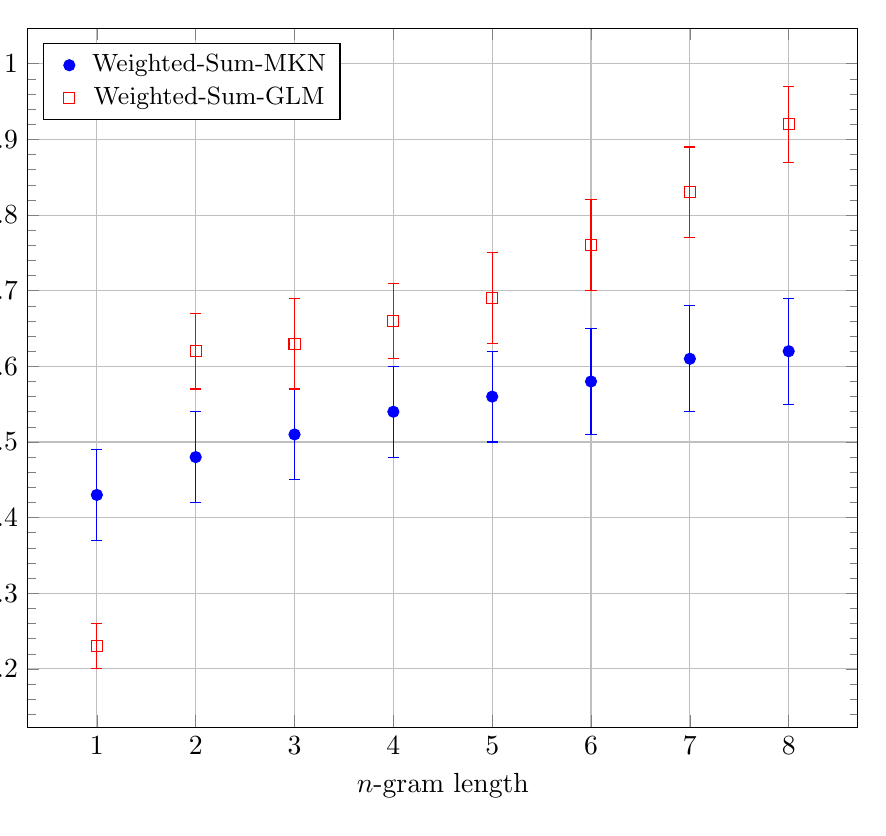
\begin{tikzpicture}[baseline, trim axis left, trim axis right]

\pgfplotscreateplotcyclelist{mkn_glm}{%
  blue,  mark size=2, mark=*,\\%
  red,   mark size=2, mark=square,\\%
}

\pgfplotsset{
  legend style = {
    legend image code/.code = {
      \draw[only marks]
        plot coordinates {
          (0.3cm,0cm)
        };
      \node at (0.15cm, 0cm) {};
      \node at (0.45cm, 0cm) {};
    },
  },
}

\begin{axis}[
%   title = {Relative Weight $\SumWeight^h_i$ Calculation Time per Probability},
  xlabel = {$n$-gram length},
  xtick = {1, ..., 8},
  ylabel = {Relative Calculation Time},
  %ymin = 0,
  minor y tick num = 4,
  grid = major,
  %enlargelimits = 0.025,
  cycle list name = mkn_glm,
  legend entries = {{\small{Weighted-Sum-MKN}}, {\small{Weighted-Sum-GLM}}},
  legend pos = north west,
  legend style = {
    row sep = 0ex,
    xshift = -0.12cm,
    yshift =  0.08cm,
  },
  width = \textwidth,
]

% MKN
\addplot+[
  only marks,
  error bars/.cd,
  y dir = both,
  y explicit,
] table [y error = stddev] {
  n ratio stddev
  1 0.43 0.06
  2 0.48 0.06
  3 0.51 0.06
  4 0.54 0.06
  5 0.56 0.06
  6 0.58 0.07
  7 0.61 0.07
  8 0.62 0.07
%  1 0.79 0.44
%  2 0.95 0.30
%  3 1.08 0.31
%  4 1.22 0.36
%  5 1.34 0.38
%  6 1.48 1.10
%  7 1.62 0.52
%  8 1.75 0.54
};

% GLM
\addplot+[
  only marks,
  error bars/.cd,
  y dir = both,
  y explicit,
] table [y error = stddev] {
  n ratio stddev
  1 0.23 0.03
  2 0.62 0.05
  3 0.63 0.06
  4 0.66 0.05
  5 0.69 0.06
  6 0.76 0.06
  7 0.83 0.06
  8 0.92 0.05
%  1  0.30  0.16
%  2  1.69  1.48
%  3  1.74  0.47
%  4  2.01  1.33
%  5  2.40  0.91
%  6  3.40  1.66
%  7  5.97  6.08
%  8 14.45 16.69
};

\end{axis}

\end{tikzpicture}
\end{document}

  \end{minipage}
  \caption{Proportion of the calculation time per probability that is used
    for the calculation of the weights $\SumWeight^h_i$.
    Given for the weighted-sum approach of both Modified Kneser-Ney Smoothing
    (MKN) and the Generalized Language Model (GLM).
    A value of \num{0.6} means that 60\% of time
    was used to calculate the weights and the remaining 40\% of time was used
    to calculate the final probability using these weights.
    Shown is the mean of the measured values with the errors bars displaying the
    standard deviation.}
  \label{fig:evaluation-weight-times}
\end{figure}

An interesting question is now: how much time of each probability calculation
is actually used to calculate the weights, and can therefore be saved by
off-loading its calculation to a pre-computation step?
\Cref{fig:evaluation-weight-times} shows this proportion for the previous
experiment.
We can see that the amount of saved work increases with $n$-gram length.
For the interesting value of $5$-grams we note a work load reduction from
about 55\% for Modified Kneser-Ney Smoothing to 70\% for the Generalized
Language Model with an application like next word prediction.

We conclude that there is no downside to the weighted-sum approach.
For Modified Kneser-Ney Smoothing it is able to calculate probabilities in
approximately the same time, while it is about twice as fast for the
Generalized Language Model.
Additionally, in the application of next word prediction,  it to further reduce
the calculation time by around 55\% respectively 70\% depending on choice
of language model.

\begin{draft}
For different percentages of seen sequences?
Number of weights per model.
\end{draft}

% ------------------------------------------------------------------------------
\section{Next Word Prediction}
\label{sec:evaluation-topkjoin}

% - - - - - - - - - - - - - - - - - - - - - - - - - - - - - - - - - - - - - - -
\subsection{Prediction Quality}
\label{subsec:evaluation-topkjoin-quality}

First we will compare the achieved prediction quality of the employed
language models.
Note that for this experiment the choice of underlying algorithm does not
matter.
The Simple Argmax, the Threshold Algorithm, and the No-Random Access Algorithm
always predict the same words, they just compute these results in different
ways.

A standard metric to evaluate the quality of a word prediction system is the
degree of \emph{normalized keystroke savings}
\parencite{Swiffin1987,Bickel2005,Trnka2011}.
They measure the percentage of keystrokes that can be omitted by using next
word prediction compared to letter-by-letter typing.
Normalized keystroke savings (NKSS) are calculate as \parencite{Trnka2011}:
\begin{equation}
  \text{NKSS} = \frac{\text{keystrokes}_\text{normal} - \text{keystrokes}_\text{with prediction}}
                     {\text{keystrokes}_\text{normal}}
\end{equation}

In the context of next word prediction we are only concerned with the keystroke
savings of entering single, independent words.
For our purpose $\text{keystrokes}_\text{normal}$ thus is the number of
characters of a word, while $\text{keystrokes}_\text{with prediction}$ is
the number of characters of a word one has to type until the system suggests
the indented word as a completion.
This however is not a clear definition: most next word prediction systems do not
only offer a single prediction after each keystroke, but a list of $k$
predictions from which the user can choose.
Measurements of normalized keystroke savings are thus inherently depend on the
choice of $k$.

There also is no clear consensus on how keystrokes are counted
\parencite{Trnka2011}.
For this thesis, we count each character as a single keystroke, independent of
case or accessibility from a normal keyboard.
Word separating characters like spaces or newlines are not considered in our
analysis, as they do not matter for next word prediction.
On top of that we did not count the process of selecting the indented word from
the list of predictions as a keystroke to enable keystroke savings to lie in the
complete range from zero to one.

\begin{table}
  \centering
  \begin{tabular}{ccc}
    \toprule
    & \multicolumn{2}{c}{Normalized Keystroke Savings} \\
    \cmidrule{2-3}
    n-gram length & \hspace{0.8cm}MKN\hspace{0.8cm} & \hspace{0.8cm}GLM\hspace{0.8cm} \\
    \midrule
    2 & 0.44 & 0.44 \\
    3 & 0.50 & 0.50 \\
    4 & 0.51 & 0.51 \\
    5 & 0.51 & 0.52 \\
    \bottomrule
  \end{tabular}
  \caption{Comparison of normalized keystroke savings for Modified Kneser-Ney
    Smoothing (MKN) and the Generalized Language Model (GLM) over varying
    $n$-gram lengths.
    A prediction was only considered valid if the intended word occurred as
    the top-$1$ prediction.}
  \label{tab:evaluation-nkss}
\end{table}

\Cref{tab:evaluation-nkss} shows our measurement of normalized keystroke
savings with the testing sequences for both considered language models.
As is apparent, the choice between Modified Kneser-Ney Smoothing and the
Generalized Language Model is largely irrelevant from a keystroke savings point
of view, at least for our experimental setup: for two significant  digits, all
values match, with the exception of the last row, which only differs slightly.
The Generalized Language Model however comes with severely higher costs in both
required space and runtime as we will see in
\cref{subsec:evaluation-topkjoin-space,subsec:evaluation-topkjoin-time}.

% - - - - - - - - - - - - - - - - - - - - - - - - - - - - - - - - - - - - - - -
\clearpage
\subsection{Space Requirements}
\label{subsec:evaluation-topkjoin-space}

Next we will measure the memory requirements of our next word prediction
system.
Again the choice of algorithm to calculate next word prediction is irrelevant.
For all algorithms we use the same data structure to store occurrence counts of
text corpora: the completion trie described in \cref{sec:completiontrie}.
This data structure is optimized for compact storage and supports all required
access types.
However the amount of necessary data varies with the employed language model.
As the Generalized Language Model also needs to keep track of the occurrence
of skipped $n$-grams, we expect it to always require more memory.

\begin{figure}
  \centering
  Completion Trie Size for $5$-gram Prediction
  \\[1.5ex]
  \begin{minipage}{0.7\textwidth}
    \centering
    \documentclass[tikz]{standalone}
\usepackage[dvipsnames,svgnames,x11names]{xcolor}
\usepackage{tikz}
\usepackage{pgfplots}
\pgfplotsset{compat = 1.12}
\usepackage[
  group-separator={,},
  exponent-product=\cdot,
  binary-units = true,
]{siunitx}
\usepackage{../thesismath}
\begin{document}
\begin{tikzpicture}[baseline, trim axis left, trim axis right]

\pgfplotscreateplotcyclelist{mkn_glm}{%
  blue,  mark size=2, mark=*,\\%
  red,   mark size=2, mark=square,\\%
}

\pgfplotsset{
  legend style = {
    legend image code/.code = {
      \draw[only marks]
        plot coordinates {
          (0.3cm,0cm)
        };
      \node at (0.15cm, 0cm) {};
      \node at (0.45cm, 0cm) {};
    },
  },
}

\sisetup{exponent-base = 2}
\begin{axis}[
%   title = {Completion Trie Size for $5$-gram Prediction},
  xlabel = {Number of Sentences},
  xmode = log,
  xtick       = {        30400,         60801,        121602,        234204,        486409},
  xticklabels = {\num{1.85e14}, \num{1.85e15}, \num{1.85e16}, \num{1.85e17}, \num{1.85e18}},
  xticklabel style = {
    inner sep = 1pt,
    anchor = north east,
    rotate = 45,
  },
  ylabel = {Memory Space [\si{\gibi\byte}]},
  %ytick = {100, 1000, 10000},
  %yticklabels = {\num{0.1}, \num{1.0}, \num{10.0}},
  ymode = log,
  log ticks with fixed point,
  %ymin = 0,
  minor y tick num = 4,
  grid = major,
  enlargelimits = 0.2,
  cycle list name = mkn_glm,
  legend entries = {{MKN}, {GLM}},
  legend pos = north west,
  width = \textwidth,
]

% MKN
\addplot+[
  only marks,
] table [y expr = \thisrow{mb}/1024] {
  n      mb
   30400  123
   60801  226
  121602  412
  234204  740
  486409 1323
};

\node [blue, yshift = 0.5ex] at ({axis cs: 30400, 0.12}) [above] {\SI{ 123}{\mebi\byte}};
\node [blue, yshift = 0.5ex] at ({axis cs: 60801, 0.22}) [above] {\SI{ 226}{\mebi\byte}};
\node [blue, yshift = 0.5ex] at ({axis cs:121602, 0.40}) [above] {\SI{ 412}{\mebi\byte}};
\node [blue, yshift = 0.5ex] at ({axis cs:234204, 0.72}) [above] {\SI{ 740}{\mebi\byte}};
\node [blue, yshift = 0.5ex] at ({axis cs:486409, 1.29}) [above] {\SI{1.29}{\gibi\byte}};

% GLM
\addplot+[
  only marks,
] table [y expr = \thisrow{mb}/1024] {
  n      mb
   30400  781
   60801 1412
  121602 2524
  234204 4458
  486409 7821
};

\node [ red, yshift = 0.5ex] at ({axis cs: 30400, 0.76}) [above] {\SI{ 781}{\mebi\byte}};
\node [ red, yshift = 0.5ex] at ({axis cs: 60801, 1.38}) [above] {\SI{1.38}{\gibi\byte}};
\node [ red, yshift = 0.5ex] at ({axis cs:121602, 2.46}) [above] {\SI{2.46}{\gibi\byte}};
\node [ red, yshift = 0.5ex] at ({axis cs:234204, 4.35}) [above] {\SI{4.35}{\gibi\byte}};
\node [ red, yshift = 0.5ex] at ({axis cs:486409, 7.64}) [above] {\SI{7.64}{\gibi\byte}};

%\addplot [blue, domain=30400:486409, samples=100]
%  {1.7e-5*x^0.857};
%\addplot [ red, domain=30400:486409, samples=100]
%  {1.4e-4*x^0.832};

\end{axis}

\end{tikzpicture}
\end{document}

  \end{minipage}
  \caption{Memory sizes of the completion tries used to store the occurrence
    counts that are required to compute $5$-gram next word prediction.
    Distinguished for Modified Kneser-Ney Smoothing (MKN) and the Generalized
    Language Model (GLM).}
  \label{fig:evaluation-trie-size}
\end{figure}

\Cref{fig:evaluation-trie-size} shows the necessary memory for each different
corpus size and each language model.
In the plot all measurement points of one language model technique lie on one
pretty clear, straight line.
Note that both axis feature logarithmic scales.
Thus the relation between the number of sentences in a corpus and the required
memory space is monomial in practice.
As the slope of the observed line is lesser than one, the power of the monomial
also has to be lass than one.
We thus conclude that the relation between increasing corpus size to the
required memory is better than linear.

For each measured corpus size, the Generalized Language Model takes roughly
six times the amount of memory.
\todo{Explainable by six times as many patterns?}
Together with the fact that its prediction quality is only very slightly better,
there is no reason for its use over Modified Kneser-Ney Smoothing.
This argument will be reinforced by comparing their runtimes.

% - - - - - - - - - - - - - - - - - - - - - - - - - - - - - - - - - - - - - - -
\clearpage
\subsection{Runtime Analysis}
\label{subsec:evaluation-topkjoin-time}

Finally we want to compare the presented next word prediction algorithms by
their runtime, as fast next word prediction algorithms were the main objective
of this thesis.
In this thesis we described three different solutions:
\begin{inparaenum}[(1)]
  \item the Simple Argmax algorithm, which calculates the probability of all
    words in a vocabulary and then selects the ones with the highest
    probabilities,
  \item the Threshold Algorithm, known from the field of top-$k$ joining,
    which utilizes sorted and random access to a sorted list of occurrence
    counts to find predictions faster, and
  \item the No-Random-Access Algorithm which works similarly but only requires
    sorted access.
\end{inparaenum}

We studied the behavior of these algorithms under two different language models
in a wide variety of settings.
We measured the runtime of each algorithm
\begin{inparaenum}[(1)]
  \item applied to Modified Kneser-Ney Smoothing and the Generalized Language
    Model,
  \item with occurrence counts from five differently sized training corpora,
  \item for $n$-gram lengths from two to five,
  \item predicting one to five words.
\end{inparaenum}
\Cref{fig:evaluation-time-nwp-mkn-corpora,fig:evaluation-time-nwp-mkn-ngram,%
  fig:evaluation-time-nwp-mkn-predictions,fig:evaluation-time-nwp-glm-corpora,%
  fig:evaluation-time-nwp-glm-ngram,fig:evaluation-time-nwp-glm-predictions}
show selected results from these experiments.

\begin{figure}[p!]
  \vspace{-0.4cm}
  \captionsetup[subfigure]{aboveskip=0cm, belowskip=-0.4cm}

  \small
  \begin{center}
    Calculation Time per top-$1$ Prediction using $5$-grams
  \end{center}

  \vspace{-0.2cm}
  \hspace{-0.16\textwidth}
  \makebox[1.32\textwidth][c]{
    \begin{subfigure}{.65\textwidth}
      \vspace{-0.25cm}
      \raggedleft
      \documentclass[tikz]{standalone}
\usepackage[dvipsnames,svgnames,x11names]{xcolor}
\usepackage{tikz}
\usepackage{pgfplots}
\usetikzlibrary{pgfplots.statistics}
\pgfplotsset{compat = 1.12}
\usepackage[
  group-separator={,},
  exponent-product=\cdot,
]{siunitx}
\usepackage{../thesismath}
\begin{document}
\begin{tikzpicture}[baseline, trim axis left, trim axis right]

\pgfplotscreateplotcyclelist{smpl}{%
  green!60!black,  mark size=1.25, mark=square,\\%
  %blue,  mark size=1.25, mark=square,\\%
  %red,   mark size=1.25, mark=square,\\%
}

\pgfplotsset{
  legend style = {
    legend image code/.code = {
      \draw[only marks]
        plot coordinates {
          (0.3cm,0cm)
        };
      \node at (0.15cm, 0cm) {};
      \node at (0.45cm, 0cm) {};
    },
  },
  boxplot/draw/average/.code = {
    % uncomment to show dotted bars for average:
    %\draw[dashed, /pgfplots/boxplot/every average/.try]
    %  (boxplot box cs:\pgfplotsboxplotvalue{average},0)
    %  --
    %  (boxplot box cs:\pgfplotsboxplotvalue{average},1)
    %  ;
  },
}

\sisetup{exponent-base = 2}
\begin{axis}[
%   title = {Calculation Time per top-$1$ Prediction using $5$-grams},
  xlabel = {Number of Unique Words},
  %xtick       = {            1,             2,             3,             4,             5},
  %xticklabels = {\num{1.85e14}, \num{1.85e15}, \num{1.85e16}, \num{1.85e17}, \num{1.85e18}},
  xtick = {50372, 70988, 98209, 133038, 178671},
  xticklabels = {\num{50000}, \num{71000}, \num{98000}, \num{133000}, \num{179000}},
  xticklabel style = {
    inner sep = 1pt,
    anchor = north east,
    rotate = 45,
  },
  ylabel = {Calcluation Time [\si{\milli\second}]},
  ymin =  265.492867,
  ymax = 4779.094746,
  scaled x ticks = false,
  scaled y ticks = false,
  minor y tick num = 4,
  ymajorgrids = true,
  boxplot/draw direction = y,
  boxplot = {
    box extend = 8000,
  },
  cycle list name = smpl,
  enlargelimits = 0.05,
  legend entries = {{SMPL-MKN}},
  legend pos = north west,
  width = \textwidth,
]

% ------------------------------------------------------------------------------

% training-5-argmaxcompare-1k-c/ngram-5-1k-SMPL-Weighted-Sum-Modified-Kneser-Ney-1
\addplot+[
  boxplot prepared = {
    %draw position = 30400,
    draw position = 50372,
    lower whisker = 265.492867,
    lower quartile = 314.299584,
    median = 502.856222,
    upper quartile = 579.864225,
    upper whisker = 976.748291,
    average = 513.082405,
  },
] table [row sep = \\, y index = 0] {
  data\\
};

% % training-5-argmaxcompare-40k-c/ngram-5-TA-Weighted-Sum-Modified-Kneser-Ney-1
% \addplot+[
%   boxplot prepared = {
%     %draw position = 30400,
%     %draw position = 50372,
%     draw position = 45372,
%     lower whisker = 0.017048,
%     lower quartile = 0.039706,
%     median = 0.058548,
%     upper quartile = 0.085849,
%     upper whisker = 0.155036,
%     average = 0.071223,
%   },
% ] table [row sep = \\, y index = 0] {
%   data\\
% };

% % training-5-argmaxcompare-40k-c/ngram-5-NRA-Weighted-Sum-Modified-Kneser-Ney-1
% \addplot+[
%   boxplot prepared = {
%     %draw position = 30400,
%     %draw position = 50372,
%     draw position = 55372,
%     lower whisker = 0.017407,
%     lower quartile = 0.042866,
%     median = 0.063964,
%     upper quartile = 0.108526,
%     upper whisker = 0.207005,
%     average = 0.367642,
%   },
% ] table [row sep = \\, y index = 0] {
%   data\\
% };

% ------------------------------------------------------------------------------

% training-4-argmaxcompare-1k-c/ngram-5-1k-SMPL-Weighted-Sum-Modified-Kneser-Ney-1
\addplot+[
  boxplot prepared = {
    %draw position = 60801,
    draw position = 70988,
    lower whisker = 385.966344,
    lower quartile = 473.753359,
    median = 758.676964,
    upper quartile = 1014.005158,
    upper whisker = 1802.043448,
    average = 800.724252,
  },
] table [row sep = \\, y index = 0] {
  data\\
};

% % training-4-argmaxcompare-40k-c/ngram-5-TA-Weighted-Sum-Modified-Kneser-Ney-1
% \addplot+[
%   boxplot prepared = {
%     %draw position = 60801,
%     %draw position = 70988,
%     draw position = 65988,
%     lower whisker = 0.019755,
%     lower quartile = 0.045715,
%     median = 0.066753,
%     upper quartile = 0.098698,
%     upper whisker = 0.178131,
%     average = 0.081448,
%   },
% ] table [row sep = \\, y index = 0] {
%   data\\
% };

% % training-4-argmaxcompare-40k-c/ngram-5-NRA-Weighted-Sum-Modified-Kneser-Ney-1
% \addplot+[
%   boxplot prepared = {
%     %draw position = 60801,
%     %draw position = 70988,
%     draw position = 75988,
%     lower whisker = 0.019593,
%     lower quartile = 0.049044,
%     median = 0.071640,
%     upper quartile = 0.117478,
%     upper whisker = 0.220049,
%     average = 0.463580,
%   },
% ] table [row sep = \\, y index = 0] {
%   data\\
% };

% ------------------------------------------------------------------------------

% training-3-argmaxcompare-1k-c/ngram-5-1k-SMPL-Weighted-Sum-Modified-Kneser-Ney-1
\addplot+[
  boxplot prepared = {
    %draw position = 121602,
    draw position = 98209,
    lower whisker = 518.403279,
    lower quartile = 898.427997,
    median = 1050.791946,
    upper quartile = 1476.127982,
    upper whisker = 2317.160040,
    average = 1156.278226,
  },
] table [row sep = \\, y index = 0] {
  data\\
};

% % training-3-argmaxcompare-40k-c/ngram-5-TA-Weighted-Sum-Modified-Kneser-Ney-1
% \addplot+[
%   boxplot prepared = {
%     %draw position = 121602,
%     %draw position = 98209,
%     draw position = 93209,
%     lower whisker = 0.020270,
%     lower quartile = 0.051889,
%     median = 0.074050,
%     upper quartile = 0.110448,
%     upper whisker = 0.198268,
%     average = 0.090352,
%   },
% ] table [row sep = \\, y index = 0] {
%   data\\
% };

% % training-3-argmaxcompare-40k-c/ngram-5-NRA-Weighted-Sum-Modified-Kneser-Ney-1
% \addplot+[
%   boxplot prepared = {
%     %draw position = 121602,
%     %draw position = 98209,
%     draw position = 103209,
%     lower whisker = 0.020295,
%     lower quartile = 0.054553,
%     median = 0.080047,
%     upper quartile = 0.132983,
%     upper whisker = 0.250549,
%     average = 0.441277,
%   },
% ] table [row sep = \\, y index = 0] {
%   data\\
% };

% ------------------------------------------------------------------------------

% training-2-argmaxcompare-1k-c/ngram-5-1k-SMPL-Weighted-Sum-Modified-Kneser-Ney-1
\addplot+[
  boxplot prepared = {
    %draw position = 2432004,
    draw position = 133038,
    lower whisker = 739.370986,
    lower quartile = 1335.713467,
    median = 1535.447582,
    upper quartile = 2146.337549,
    upper whisker = 3356.148393,
    average = 1727.968135,
  },
] table [row sep = \\, y index = 0] {
  data\\
};

% % training-2-argmaxcompare-40k-c/ngram-5-TA-Weighted-Sum-Modified-Kneser-Ney-1
% \addplot+[
%   boxplot prepared = {
%     %draw position = 2432004,
%     draw position = 133038,
%     draw position = 128038,
%     lower whisker = 0.021501,
%     lower quartile = 0.059342,
%     median = 0.084170,
%     upper quartile = 0.124255,
%     upper whisker = 0.221622,
%     average = 0.101046,
%   },
% ] table [row sep = \\, y index = 0] {
%   data\\
% };

% % training-2-argmaxcompare-40k-c/ngram-5-NRA-Weighted-Sum-Modified-Kneser-Ney-1
% \addplot+[
%   boxplot prepared = {
%     %draw position = 2432004,
%     %draw position = 133038,
%     draw position = 138038,
%     lower whisker = 0.019813,
%     lower quartile = 0.062182,
%     median = 0.092578,
%     upper quartile = 0.150630,
%     upper whisker = 0.283221,
%     average = 0.553668,
%   },
% ] table [row sep = \\, y index = 0] {
%   data\\
% };

% ------------------------------------------------------------------------------

% training-1-argmaxcompare-1k-c/ngram-5-1k-SMPL-Weighted-Sum-Modified-Kneser-Ney-1
\addplot+[
  boxplot prepared = {
    %draw position = 486409,
    draw position = 178671,
    lower whisker = 1002.784867,
    lower quartile = 1886.653179,
    median = 2408.640801,
    upper quartile = 3109.965427,
    upper whisker = 4779.094746,
    average = 2527.778769,
  },
] table [row sep = \\, y index = 0] {
  data\\
};

% % training-1-argmaxcompare-40k-c/ngram-5-TA-Weighted-Sum-Modified-Kneser-Ney-1
% \addplot+[
%   boxplot prepared = {
%     %draw position = 486409,
%     %draw position = 178671,
%     draw position = 173671,
%     lower whisker = 0.022592,
%     lower quartile = 0.066967,
%     median = 0.094754,
%     upper quartile = 0.136932,
%     upper whisker = 0.241880,
%     average = 0.111001,
%   },
% ] table [row sep = \\, y index = 0] {
%   data\\
% };

% % training-1-argmaxcompare-40k-c/ngram-5-NRA-Weighted-Sum-Modified-Kneser-Ney-1
% \addplot+[
%   boxplot prepared = {
%     %draw position = 486409,
%     %draw position = 178671,
%     draw position = 183671,
%     lower whisker = 0.023497,
%     lower quartile = 0.073006,
%     median = 0.110507,
%     upper quartile = 0.174697,
%     upper whisker = 0.327149,
%     average = 0.608050,
%   },
% ] table [row sep = \\, y index = 0] {
%   data\\
% };

% \draw [blue]
%   ({axis cs: 45372, 0.058548}) --
%   ({axis cs: 65988, 0.066753}) --
%   ({axis cs: 93209, 0.074050}) --
%   ({axis cs:133038, 0.084170}) --
%   ({axis cs:173671, 0.094754})
% ;
%
% \draw [red]
%   ({axis cs: 55372, 0.063964}) --
%   ({axis cs: 75988, 0.071640}) --
%   ({axis cs:103209, 0.080047}) --
%   ({axis cs:138038, 0.092578}) --
%   ({axis cs:183671, 0.110507})
% ;

\end{axis}

\end{tikzpicture}
\end{document}

      \subcaption{}
      \label{fig:evaluation-time-nwp-mkn-corpora-smpl}
    \end{subfigure}
    \hspace{.02\textwidth}
    \begin{subfigure}{.65\textwidth}
      \raggedright
      \documentclass[tikz]{standalone}
\usepackage[dvipsnames,svgnames,x11names]{xcolor}
\usepackage{tikz}
\usepackage{pgfplots}
\usetikzlibrary{pgfplots.statistics}
\pgfplotsset{compat = 1.12}
\usepackage[
  group-separator={,},
  exponent-product=\cdot,
]{siunitx}
\usepackage{../thesismath}
\begin{document}
\begin{tikzpicture}[baseline, trim axis left, trim axis right]

\pgfplotscreateplotcyclelist{ta_nra}{%
  blue,  mark size=1.25, mark=square,\\%
  red,   mark size=1.25, mark=square,\\%
}

\pgfplotsset{
  legend style = {
    legend image code/.code = {
      \draw[only marks]
        plot coordinates {
          (0.3cm,0cm)
        };
      \node at (0.15cm, 0cm) {};
      \node at (0.45cm, 0cm) {};
    },
  },
  boxplot/draw/average/.code = {
    % uncomment to show dotted bars for average:
    %\draw[dashed, /pgfplots/boxplot/every average/.try]
    %  (boxplot box cs:\pgfplotsboxplotvalue{average},0)
    %  --
    %  (boxplot box cs:\pgfplotsboxplotvalue{average},1)
    %  ;
  },
}

\sisetup{exponent-base = 2}
\begin{axis}[
%   title = {Calculation Time per top-$1$ Prediction using $5$-grams},
  xlabel = {Number of Unique Words},
  %xtick       = {            1,             2,             3,             4,             5},
  %xticklabels = {\num{1.85e14}, \num{1.85e15}, \num{1.85e16}, \num{1.85e17}, \num{1.85e18}},
  xtick = {50372, 70988, 98209, 133038, 178671},
  xticklabels = {\num{50000}, \num{71000}, \num{98000}, \num{133000}, \num{179000}},
  xticklabel style = {
    inner sep = 1pt,
    anchor = north east,
    rotate = 45,
  },
  ylabel = {Calcluation Time [\si{\milli\second}]},
  yticklabel pos = right,
  ymin = 0.01704,
  ymax = 0.32714,
  scaled x ticks = false,
  scaled y ticks = false,
  minor y tick num = 4,
  y tick label style = {
    /pgf/number format/fixed,
    /pgf/number format/fixed zerofill,
  },
  ymajorgrids = true,
  boxplot/draw direction = y,
  boxplot = {
    box extend = 8000,
  },
  cycle list name = ta_nra,
  enlargelimits = 0.05,
  legend entries = {{TA-MKN}, {NRA-MKN}},
  legend pos = north west,
  width = \textwidth,
]

% ------------------------------------------------------------------------------

% % training-5-argmaxcompare-1k-c/ngram-5-1k-SMPL-Weighted-Sum-Modified-Kneser-Ney-1
% \addplot+[
%   boxplot prepared = {
%     %draw position = 30400,
%     draw position = 50372,
%     lower whisker = 265.492867,
%     lower quartile = 314.299584,
%     median = 502.856222,
%     upper quartile = 579.864225,
%     upper whisker = 976.748291,
%     average = 513.082405,
%   },
% ] table [row sep = \\, y index = 0] {
%   data\\
% };

% training-5-argmaxcompare-40k-c/ngram-5-TA-Weighted-Sum-Modified-Kneser-Ney-1
\addplot+[
  boxplot prepared = {
    %draw position = 30400,
    %draw position = 50372,
    draw position = 45372,
    lower whisker = 0.017048,
    lower quartile = 0.039706,
    median = 0.058548,
    upper quartile = 0.085849,
    upper whisker = 0.155036,
    average = 0.071223,
  },
] table [row sep = \\, y index = 0] {
  data\\
};

% training-5-argmaxcompare-40k-c/ngram-5-NRA-Weighted-Sum-Modified-Kneser-Ney-1
\addplot+[
  boxplot prepared = {
    %draw position = 30400,
    %draw position = 50372,
    draw position = 55372,
    lower whisker = 0.017407,
    lower quartile = 0.042866,
    median = 0.063964,
    upper quartile = 0.108526,
    upper whisker = 0.207005,
    average = 0.367642,
  },
] table [row sep = \\, y index = 0] {
  data\\
};

% ------------------------------------------------------------------------------

% % training-4-argmaxcompare-1k-c/ngram-5-1k-SMPL-Weighted-Sum-Modified-Kneser-Ney-1
% \addplot+[
%   boxplot prepared = {
%     %draw position = 60801,
%     draw position = 70988,
%     lower whisker = 385.966344,
%     lower quartile = 473.753359,
%     median = 758.676964,
%     upper quartile = 1014.005158,
%     upper whisker = 1802.043448,
%     average = 800.724252,
%   },
% ] table [row sep = \\, y index = 0] {
%   data\\
% };

% training-4-argmaxcompare-40k-c/ngram-5-TA-Weighted-Sum-Modified-Kneser-Ney-1
\addplot+[
  boxplot prepared = {
    %draw position = 60801,
    %draw position = 70988,
    draw position = 65988,
    lower whisker = 0.019755,
    lower quartile = 0.045715,
    median = 0.066753,
    upper quartile = 0.098698,
    upper whisker = 0.178131,
    average = 0.081448,
  },
] table [row sep = \\, y index = 0] {
  data\\
};

% training-4-argmaxcompare-40k-c/ngram-5-NRA-Weighted-Sum-Modified-Kneser-Ney-1
\addplot+[
  boxplot prepared = {
    %draw position = 60801,
    %draw position = 70988,
    draw position = 75988,
    lower whisker = 0.019593,
    lower quartile = 0.049044,
    median = 0.071640,
    upper quartile = 0.117478,
    upper whisker = 0.220049,
    average = 0.463580,
  },
] table [row sep = \\, y index = 0] {
  data\\
};

% ------------------------------------------------------------------------------

% % training-3-argmaxcompare-1k-c/ngram-5-1k-SMPL-Weighted-Sum-Modified-Kneser-Ney-1
% \addplot+[
%   boxplot prepared = {
%     %draw position = 121602,
%     draw position = 98209,
%     lower whisker = 518.403279,
%     lower quartile = 898.427997,
%     median = 1050.791946,
%     upper quartile = 1476.127982,
%     upper whisker = 2317.160040,
%     average = 1156.278226,
%   },
% ] table [row sep = \\, y index = 0] {
%   data\\
% };

% training-3-argmaxcompare-40k-c/ngram-5-TA-Weighted-Sum-Modified-Kneser-Ney-1
\addplot+[
  boxplot prepared = {
    %draw position = 121602,
    %draw position = 98209,
    draw position = 93209,
    lower whisker = 0.020270,
    lower quartile = 0.051889,
    median = 0.074050,
    upper quartile = 0.110448,
    upper whisker = 0.198268,
    average = 0.090352,
  },
] table [row sep = \\, y index = 0] {
  data\\
};

% training-3-argmaxcompare-40k-c/ngram-5-NRA-Weighted-Sum-Modified-Kneser-Ney-1
\addplot+[
  boxplot prepared = {
    %draw position = 121602,
    %draw position = 98209,
    draw position = 103209,
    lower whisker = 0.020295,
    lower quartile = 0.054553,
    median = 0.080047,
    upper quartile = 0.132983,
    upper whisker = 0.250549,
    average = 0.441277,
  },
] table [row sep = \\, y index = 0] {
  data\\
};

% ------------------------------------------------------------------------------

% % training-2-argmaxcompare-1k-c/ngram-5-1k-SMPL-Weighted-Sum-Modified-Kneser-Ney-1
% \addplot+[
%   boxplot prepared = {
%     %draw position = 2432004,
%     draw position = 133038,
%     lower whisker = 739.370986,
%     lower quartile = 1335.713467,
%     median = 1535.447582,
%     upper quartile = 2146.337549,
%     upper whisker = 3356.148393,
%     average = 1727.968135,
%   },
% ] table [row sep = \\, y index = 0] {
%   data\\
% };

% training-2-argmaxcompare-40k-c/ngram-5-TA-Weighted-Sum-Modified-Kneser-Ney-1
\addplot+[
  boxplot prepared = {
    %draw position = 2432004,
    draw position = 133038,
    draw position = 128038,
    lower whisker = 0.021501,
    lower quartile = 0.059342,
    median = 0.084170,
    upper quartile = 0.124255,
    upper whisker = 0.221622,
    average = 0.101046,
  },
] table [row sep = \\, y index = 0] {
  data\\
};

% training-2-argmaxcompare-40k-c/ngram-5-NRA-Weighted-Sum-Modified-Kneser-Ney-1
\addplot+[
  boxplot prepared = {
    %draw position = 2432004,
    %draw position = 133038,
    draw position = 138038,
    lower whisker = 0.019813,
    lower quartile = 0.062182,
    median = 0.092578,
    upper quartile = 0.150630,
    upper whisker = 0.283221,
    average = 0.553668,
  },
] table [row sep = \\, y index = 0] {
  data\\
};

% ------------------------------------------------------------------------------

% % training-1-argmaxcompare-1k-c/ngram-5-1k-SMPL-Weighted-Sum-Modified-Kneser-Ney-1
% \addplot+[
%   boxplot prepared = {
%     %draw position = 486409,
%     draw position = 178671,
%     lower whisker = 1002.784867,
%     lower quartile = 1886.653179,
%     median = 2408.640801,
%     upper quartile = 3109.965427,
%     upper whisker = 4779.094746,
%     average = 2527.778769,
%   },
% ] table [row sep = \\, y index = 0] {
%   data\\
% };

% training-1-argmaxcompare-40k-c/ngram-5-TA-Weighted-Sum-Modified-Kneser-Ney-1
\addplot+[
  boxplot prepared = {
    %draw position = 486409,
    %draw position = 178671,
    draw position = 173671,
    lower whisker = 0.022592,
    lower quartile = 0.066967,
    median = 0.094754,
    upper quartile = 0.136932,
    upper whisker = 0.241880,
    average = 0.111001,
  },
] table [row sep = \\, y index = 0] {
  data\\
};

% training-1-argmaxcompare-40k-c/ngram-5-NRA-Weighted-Sum-Modified-Kneser-Ney-1
\addplot+[
  boxplot prepared = {
    %draw position = 486409,
    %draw position = 178671,
    draw position = 183671,
    lower whisker = 0.023497,
    lower quartile = 0.073006,
    median = 0.110507,
    upper quartile = 0.174697,
    upper whisker = 0.327149,
    average = 0.608050,
  },
] table [row sep = \\, y index = 0] {
  data\\
};

% \draw [blue]
%   ({axis cs: 45372, 0.058548}) --
%   ({axis cs: 65988, 0.066753}) --
%   ({axis cs: 93209, 0.074050}) --
%   ({axis cs:133038, 0.084170}) --
%   ({axis cs:173671, 0.094754})
% ;
%
% \draw [red]
%   ({axis cs: 55372, 0.063964}) --
%   ({axis cs: 75988, 0.071640}) --
%   ({axis cs:103209, 0.080047}) --
%   ({axis cs:138038, 0.092578}) --
%   ({axis cs:183671, 0.110507})
% ;

\end{axis}

\end{tikzpicture}
\end{document}

      \subcaption{}
      \label{fig:evaluation-time-nwp-mkn-corpora-ta-nra}
    \end{subfigure}
  }
  \normalsize
  \caption{Time to calculate one top-$1$ word prediction query using
    $5$-grams over varying training corpus sizes for Modified Kneser-Ney
    Smoothing.}
  \label{fig:evaluation-time-nwp-mkn-corpora}

  \small
  \vspace{-3ex}
  \begin{center}
    \mbox{Calculation Time per top-$1$ Prediction on Corpus with \num{179000} Unique Words}
  \end{center}

  \vspace{-0.2cm}
  \hspace{-0.16\textwidth}
  \makebox[1.32\textwidth][c]{
    \begin{subfigure}{.65\textwidth}
      \raggedleft
      \documentclass[tikz]{standalone}
\usepackage[dvipsnames,svgnames,x11names]{xcolor}
\usepackage{tikz}
\usepackage{pgfplots}
\usetikzlibrary{pgfplots.statistics}
\pgfplotsset{compat = 1.12}
\usepackage[
  group-separator={,},
  exponent-product=\cdot,
]{siunitx}
\usepackage{../thesismath}
\begin{document}
\begin{tikzpicture}[baseline, trim axis left, trim axis right]

\pgfplotscreateplotcyclelist{smpl}{%
  green!60!black,  mark size=1.25, mark=square,\\%
  %blue,  mark size=1.25, mark=square,\\%
  %red,   mark size=1.25, mark=square,\\%
}

\pgfplotsset{
  legend style = {
    legend image code/.code = {
      \draw[only marks]
        plot coordinates {
          (0.3cm,0cm)
        };
      \node at (0.15cm, 0cm) {};
      \node at (0.45cm, 0cm) {};
    },
  },
  boxplot/draw/average/.code = {
    % uncomment to show dotted bars for average:
    %\draw[dashed, /pgfplots/boxplot/every average/.try]
    %  (boxplot box cs:\pgfplotsboxplotvalue{average},0)
    %  --
    %  (boxplot box cs:\pgfplotsboxplotvalue{average},1)
    %  ;
  },
}

\sisetup{exponent-base = 2}
\begin{axis}[
%   title = {Calculation Time per top-$1$ Prediction using $5$-grams},
  xlabel = {$n$-gram length},
  xtick = {2, ..., 5},
  ylabel = {Calcluation Time [\si{\milli\second}]},
  ymin = 1000.650586,
  ymax = 4779.094746,
  scaled x ticks = false,
  scaled y ticks = false,
  minor y tick num = 4,
  ymajorgrids = true,
  boxplot/draw direction = y,
  boxplot = {
    box extend = 0.4,
  },
  cycle list name = smpl,
  enlargelimits = 0.05,
  legend entries = {{SMPL-MKN}},
  legend pos = north west,
  width = \textwidth,
]

% ------------------------------------------------------------------------------

% ngram-2-1k-SMPL-Weighted-Sum-Modified-Kneser-Ney-1
\addplot+[
  boxplot prepared = {
    draw position = 2,
    lower whisker = 1000.650586,
    lower quartile = 1106.196861,
    median = 1141.434591,
    upper quartile = 1180.474463,
    upper whisker = 1291.326611,
    average = 1148.429712,
  },
] table [row sep = \\, y index = 0] {
  data\\
};

% ------------------------------------------------------------------------------

% ngram-3-1k-SMPL-Weighted-Sum-Modified-Kneser-Ney-1
\addplot+[
  boxplot prepared = {
    draw position = 3,
    lower whisker = 1560.253230,
    lower quartile = 1818.281721,
    median = 1938.952003,
    upper quartile = 2041.899413,
    upper whisker = 2373.453019,
    average = 1864.099853,
  },
] table [row sep = \\, y index = 0] {
  data\\
};

% ------------------------------------------------------------------------------

% ngram-4-1k-SMPL-Weighted-Sum-Modified-Kneser-Ney-1
\addplot+[
  boxplot prepared = {
    draw position = 4,
    lower whisker = 1004.059583,
    lower quartile = 1908.680681,
    median = 2343.640128,
    upper quartile = 2887.303063,
    upper whisker = 3632.671078,
    average = 2327.827820,
  },
] table [row sep = \\, y index = 0] {
  data\\
};

% ------------------------------------------------------------------------------

% ngram-5-1k-SMPL-Weighted-Sum-Modified-Kneser-Ney-1
\addplot+[
  boxplot prepared = {
    draw position = 5,
    lower whisker = 1002.784867,
    lower quartile = 1886.653179,
    median = 2408.640801,
    upper quartile = 3109.965427,
    upper whisker = 4779.094746,
    average = 2527.778769,
  },
] table [row sep = \\, y index = 0] {
  data\\
};

\end{axis}

\end{tikzpicture}
\end{document}

      \subcaption{}
      \label{fig:evaluation-time-nwp-mkn-ngram-smpl}
    \end{subfigure}
    \hspace{.02\textwidth}
    \begin{subfigure}{.65\textwidth}
      \raggedright
      \documentclass[tikz]{standalone}
\usepackage[dvipsnames,svgnames,x11names]{xcolor}
\usepackage{tikz}
\usepackage{pgfplots}
\usetikzlibrary{pgfplots.statistics}
\pgfplotsset{compat = 1.12}
\usepackage[
  group-separator={,},
  exponent-product=\cdot,
]{siunitx}
\usepackage{../thesismath}
\begin{document}
\begin{tikzpicture}[baseline, trim axis left, trim axis right]

\pgfplotscreateplotcyclelist{ta_nra}{%
  blue,  mark size=1.25, mark=square,\\%
  red,   mark size=1.25, mark=square,\\%
}

\pgfplotsset{
  legend style = {
    legend image code/.code = {
      \draw[only marks]
        plot coordinates {
          (0.3cm,0cm)
        };
      \node at (0.15cm, 0cm) {};
      \node at (0.45cm, 0cm) {};
    },
  },
  boxplot/draw/average/.code = {
    % uncomment to show dotted bars for average:
    %\draw[dashed, /pgfplots/boxplot/every average/.try]
    %  (boxplot box cs:\pgfplotsboxplotvalue{average},0)
    %  --
    %  (boxplot box cs:\pgfplotsboxplotvalue{average},1)
    %  ;
  },
}

\sisetup{exponent-base = 2}
\begin{axis}[
%   title = {Calculation Time per top-$1$ Prediction using $5$-grams},
  xlabel = {$n$-gram length},
  xtick = {2, ..., 5},
  ylabel = {Calcluation Time [\si{\milli\second}]},
  yticklabel pos = right,
  ymin = 0.008240,
  ymax = 0.327149,
  scaled x ticks = false,
  scaled y ticks = false,
  minor y tick num = 4,
  y tick label style = {
    /pgf/number format/fixed,
    /pgf/number format/fixed zerofill,
  },
  ymajorgrids = true,
  boxplot/draw direction = y,
  boxplot = {
    box extend = 0.4,
  },
  cycle list name = ta_nra,
  enlargelimits = 0.05,
  legend entries = {{TA-MKN}, {NRA-MKN}},
  legend pos = north west,
  width = \textwidth,
]

% ------------------------------------------------------------------------------

% ngram-2-TA-Weighted-Sum-Modified-Kneser-Ney-1
\addplot+[
  boxplot prepared = {
    draw position = 1.75,
    lower whisker = 0.008240,
    lower quartile = 0.019236,
    median = 0.023249,
    upper quartile = 0.028564,
    upper whisker = 0.042556,
    average = 0.026380,
  },
] table [row sep = \\, y index = 0] {
  data\\
};

% ngram-2-NRA-Weighted-Sum-Modified-Kneser-Ney-1
\addplot+[
  boxplot prepared = {
    draw position = 2.25,
    lower whisker = 0.008994,
    lower quartile = 0.016838,
    median = 0.020272,
    upper quartile = 0.024743,
    upper whisker = 0.036600,
    average = 0.081141,
  },
] table [row sep = \\, y index = 0] {
  data\\
};

% ------------------------------------------------------------------------------

% ngram-3-TA-Weighted-Sum-Modified-Kneser-Ney-1
\addplot+[
  boxplot prepared = {
    draw position = 2.75,
    lower whisker = 0.014419,
    lower quartile = 0.044061,
    median = 0.055573,
    upper quartile = 0.068383,
    upper whisker = 0.104854,
    average = 0.059373,
  },
] table [row sep = \\, y index = 0] {
  data\\
};

% ngram-3-NRA-Weighted-Sum-Modified-Kneser-Ney-1
\addplot+[
  boxplot prepared = {
    draw position = 3.25,
    lower whisker = 0.014226,
    lower quartile = 0.043054,
    median = 0.054306,
    upper quartile = 0.071823,
    upper whisker = 0.114975,
    average = 0.358936,
  },
] table [row sep = \\, y index = 0] {
  data\\
};

% ------------------------------------------------------------------------------

% ngram-4-TA-Weighted-Sum-Modified-Kneser-Ney-1
\addplot+[
  boxplot prepared = {
    draw position = 3.75,
    lower whisker = 0.018174,
    lower quartile = 0.059696,
    median = 0.083289,
    upper quartile = 0.112339,
    upper whisker = 0.191289,
    average = 0.092666,
  },
] table [row sep = \\, y index = 0] {
  data\\
};

% ngram-4-NRA-Weighted-Sum-Modified-Kneser-Ney-1
\addplot+[
  boxplot prepared = {
    draw position = 4.25,
    lower whisker = 0.017010,
    lower quartile = 0.062055,
    median = 0.090013,
    upper quartile = 0.128487,
    upper whisker = 0.228120,
    average = 0.569383,
  },
] table [row sep = \\, y index = 0] {
  data\\
};

% ------------------------------------------------------------------------------

% ngram-5-TA-Weighted-Sum-Modified-Kneser-Ney-1
\addplot+[
  boxplot prepared = {
    draw position = 4.75,
    lower whisker = 0.022592,
    lower quartile = 0.066967,
    median = 0.094754,
    upper quartile = 0.136932,
    upper whisker = 0.241880,
    average = 0.111001,
  },
] table [row sep = \\, y index = 0] {
  data\\
};

% ngram-5-NRA-Weighted-Sum-Modified-Kneser-Ney-1
\addplot+[
  boxplot prepared = {
    draw position = 5.25,
    lower whisker = 0.023497,
    lower quartile = 0.073006,
    median = 0.110507,
    upper quartile = 0.174697,
    upper whisker = 0.327149,
    average = 0.608050,
  },
] table [row sep = \\, y index = 0] {
  data\\
};

\end{axis}

\end{tikzpicture}
\end{document}

      \subcaption{}
      \label{fig:evaluation-time-nwp-mkn-ngram-ta-nra}
    \end{subfigure}
  }
  \normalsize
  \caption{Time to calculate one top-$1$ word prediction query with language
    model $n$-gram length varied from two to five for Modified Kneser-Ney
    Smoothing. Calculated on the \texttt{Training-100\%} corpus.}
  \label{fig:evaluation-time-nwp-mkn-ngram}

  \small
  \vspace{-3ex}
  \begin{center}
    \mbox{\hspace{-0.8cm}Calculation Time per Prediction using $5$-grams on Corpus with \num{179000} Unique Words}
  \end{center}

  \vspace{-0.2cm}
  \hspace{-0.16\textwidth}
  \makebox[1.32\textwidth][c]{
    \begin{subfigure}{.65\textwidth}
      \vspace{-0.25cm}
      \raggedleft
      \documentclass[tikz]{standalone}
\usepackage[dvipsnames,svgnames,x11names]{xcolor}
\usepackage{tikz}
\usepackage{pgfplots}
\usetikzlibrary{pgfplots.statistics}
\pgfplotsset{compat = 1.12}
\usepackage[
  group-separator={,},
  exponent-product=\cdot,
]{siunitx}
\usepackage{../thesismath}
\begin{document}
\begin{tikzpicture}[baseline, trim axis left, trim axis right]

\pgfplotscreateplotcyclelist{smpl}{%
  green!60!black,  mark size=1.25, mark=square,\\%
  %blue,  mark size=1.25, mark=square,\\%
  %red,   mark size=1.25, mark=square,\\%
}

\pgfplotsset{
  legend style = {
    legend image code/.code = {
      \draw[only marks]
        plot coordinates {
          (0.3cm,0cm)
        };
      \node at (0.15cm, 0cm) {};
      \node at (0.45cm, 0cm) {};
    },
  },
  boxplot/draw/average/.code = {
    % uncomment to show dotted bars for average:
    %\draw[dashed, /pgfplots/boxplot/every average/.try]
    %  (boxplot box cs:\pgfplotsboxplotvalue{average},0)
    %  --
    %  (boxplot box cs:\pgfplotsboxplotvalue{average},1)
    %  ;
  },
}

\sisetup{exponent-base = 2}
\begin{axis}[
%   title = {Calculation Time per top-$1$ Prediction using $5$-grams},
  xlabel = {Number of Predictions $k$},
  xtick = {1, ..., 5},
  ylabel = {Calcluation Time [\si{\milli\second}]},
  ymin = 972.638274,
  ymax = 4825.863350,
  scaled x ticks = false,
  scaled y ticks = false,
  minor y tick num = 4,
  ymajorgrids = true,
  boxplot/draw direction = y,
  boxplot = {
    box extend = 0.4,
  },
  cycle list name = smpl,
  enlargelimits = 0.05,
  legend entries = {{SMPL-MKN}},
  legend pos = north west,
  width = \textwidth,
]

% ------------------------------------------------------------------------------

% ngram-5-1k-SMPL-Weighted-Sum-Modified-Kneser-Ney-1
\addplot+[
  boxplot prepared = {
    draw position = 1,
    lower whisker = 1002.784867,
    lower quartile = 1886.653179,
    median = 2408.640801,
    upper quartile = 3109.965427,
    upper whisker = 4779.094746,
    average = 2527.778769,
  },
] table [row sep = \\, y index = 0] {
  data\\
};

% ------------------------------------------------------------------------------

% ngram-5-1k-SMPL-Weighted-Sum-Modified-Kneser-Ney-2
\addplot+[
  boxplot prepared = {
    draw position = 2,
    lower whisker = 1004.600336,
    lower quartile = 1888.090747,
    median = 2411.737365,
    upper quartile = 3109.464697,
    upper whisker = 4825.863350,
    average = 2527.347277,
  },
] table [row sep = \\, y index = 0] {
  data\\
};

% ------------------------------------------------------------------------------

% ngram-5-1k-SMPL-Weighted-Sum-Modified-Kneser-Ney-3
\addplot+[
  boxplot prepared = {
    draw position = 3,
    lower whisker = 972.638274,
    lower quartile = 1890.276163,
    median = 2400.725615,
    upper quartile = 3106.366882,
    upper whisker = 4740.173843,
    average = 2530.697348,
  },
] table [row sep = \\, y index = 0] {
  data\\
};

% ------------------------------------------------------------------------------

% ngram-5-1k-SMPL-Weighted-Sum-Modified-Kneser-Ney-4
\addplot+[
  boxplot prepared = {
    draw position = 4,
    lower whisker = 1008.249732,
    lower quartile = 1891.941958,
    median = 2408.381193,
    upper quartile = 3122.117807,
    upper whisker = 4808.688449,
    average = 2533.374697,
  },
] table [row sep = \\, y index = 0] {
  data\\
};

% ------------------------------------------------------------------------------

% ngram-5-1k-SMPL-Weighted-Sum-Modified-Kneser-Ney-5
\addplot+[
  boxplot prepared = {
    draw position = 5,
    lower whisker = 1007.382287,
    lower quartile = 1895.512416,
    median = 2421.225549,
    upper quartile = 3101.403215,
    upper whisker = 4756.829385,
    average = 2533.107267,
  },
] table [row sep = \\, y index = 0] {
  data\\
};

\end{axis}

\end{tikzpicture}
\end{document}

      \subcaption{}
      \label{fig:evaluation-time-nwp-mkn-predictions-smpl}
    \end{subfigure}
    \hspace{.02\textwidth}
    \begin{subfigure}{.65\textwidth}
      \raggedright
      \documentclass[tikz]{standalone}
\usepackage[dvipsnames,svgnames,x11names]{xcolor}
\usepackage{tikz}
\usepackage{pgfplots}
\usetikzlibrary{pgfplots.statistics}
\pgfplotsset{compat = 1.12}
\usepackage[
  group-separator={,},
  exponent-product=\cdot,
]{siunitx}
\usepackage{../thesismath}
\begin{document}
\begin{tikzpicture}[baseline, trim axis left, trim axis right]

\pgfplotscreateplotcyclelist{ta_nra}{%
  blue,  mark size=1.25, mark=square,\\%
  red,   mark size=1.25, mark=square,\\%
}

\pgfplotsset{
  legend style = {
    legend image code/.code = {
      \draw[only marks]
        plot coordinates {
          (0.3cm,0cm)
        };
      \node at (0.15cm, 0cm) {};
      \node at (0.45cm, 0cm) {};
    },
  },
  boxplot/draw/average/.code = {
    % uncomment to show dotted bars for average:
    %\draw[dashed, /pgfplots/boxplot/every average/.try]
    %  (boxplot box cs:\pgfplotsboxplotvalue{average},0)
    %  --
    %  (boxplot box cs:\pgfplotsboxplotvalue{average},1)
    %  ;
  },
}

\sisetup{exponent-base = 2}
\begin{axis}[
%   title = {Calculation Time per top-$1$ Prediction using $5$-grams},
  xlabel = {Number of Predictions $k$},
  xtick = {1, ..., 5},
  ylabel = {Calcluation Time [\si{\milli\second}]},
  yticklabel pos = right,
  ymin = 0.017174,
  ymax = 2.495233,
  scaled x ticks = false,
  scaled y ticks = false,
  minor y tick num = 4,
  y tick label style = {
    /pgf/number format/fixed,
    /pgf/number format/fixed zerofill,
  },
  ymajorgrids = true,
  boxplot/draw direction = y,
  boxplot = {
    box extend = 0.4,
  },
  cycle list name = ta_nra,
  enlargelimits = 0.05,
  legend entries = {{TA-MKN}, {NRA-MKN}},
  legend pos = north west,
  width = \textwidth,
]

% ------------------------------------------------------------------------------

% ngram-5-TA-Weighted-Sum-Modified-Kneser-Ney-1
\addplot+[
  boxplot prepared = {
    draw position = 0.75,
    lower whisker = 0.022592,
    lower quartile = 0.066967,
    median = 0.094754,
    upper quartile = 0.136932,
    upper whisker = 0.241880,
    average = 0.111001,
  },
] table [row sep = \\, y index = 0] {
  data\\
};

% ngram-5-NRA-Weighted-Sum-Modified-Kneser-Ney-1
\addplot+[
  boxplot prepared = {
    draw position = 1.25,
    lower whisker = 0.023497,
    lower quartile = 0.073006,
    median = 0.110507,
    upper quartile = 0.174697,
    upper whisker = 0.327149,
    average = 0.608050,
  },
] table [row sep = \\, y index = 0] {
  data\\
};

% ------------------------------------------------------------------------------

% ngram-5-TA-Weighted-Sum-Modified-Kneser-Ney-2
\addplot+[
  boxplot prepared = {
    draw position = 1.75,
    lower whisker = 0.017174,
    lower quartile = 0.057553,
    median = 0.087607,
    upper quartile = 0.130334,
    upper whisker = 0.239397,
    average = 0.104911,
  },
] table [row sep = \\, y index = 0] {
  data\\
};

% ngram-5-NRA-Weighted-Sum-Modified-Kneser-Ney-2
\addplot+[
  boxplot prepared = {
    draw position = 2.25,
    lower whisker = 0.019245,
    lower quartile = 0.057781,
    median = 0.104145,
    upper quartile = 0.214235,
    upper whisker = 0.448883,
    average = 1.590877,
  },
] table [row sep = \\, y index = 0] {
  data\\
};

% ------------------------------------------------------------------------------

% ngram-5-TA-Weighted-Sum-Modified-Kneser-Ney-3
\addplot+[
  boxplot prepared = {
    draw position = 2.75,
    lower whisker = 0.019819,
    lower quartile = 0.069181,
    median = 0.104469,
    upper quartile = 0.154520,
    upper whisker = 0.282474,
    average = 0.124390,
  },
] table [row sep = \\, y index = 0] {
  data\\
};

% ngram-5-NRA-Weighted-Sum-Modified-Kneser-Ney-3
\addplot+[
  boxplot prepared = {
    draw position = 3.25,
    lower whisker = 0.023286,
    lower quartile = 0.080929,
    median = 0.164101,
    upper quartile = 0.413183,
    upper whisker = 0.911395,
    average = 3.037460,
  },
] table [row sep = \\, y index = 0] {
  data\\
};

% ------------------------------------------------------------------------------

% ngram-5-TA-Weighted-Sum-Modified-Kneser-Ney-4
\addplot+[
  boxplot prepared = {
    draw position = 3.75,
    lower whisker = 0.024035,
    lower quartile = 0.081815,
    median = 0.122768,
    upper quartile = 0.178168,
    upper whisker = 0.322649,
    average = 0.145260,
  },
] table [row sep = \\, y index = 0] {
  data\\
};

% ngram-5-NRA-Weighted-Sum-Modified-Kneser-Ney-4
\addplot+[
  boxplot prepared = {
    draw position = 4.25,
    lower whisker = 0.025667,
    lower quartile = 0.111674,
    median = 0.246667,
    upper quartile = 0.699538,
    upper whisker = 1.581046,
    average = 4.795189,
  },
] table [row sep = \\, y index = 0] {
  data\\
};

% ------------------------------------------------------------------------------

% ngram-5-TA-Weighted-Sum-Modified-Kneser-Ney-5
\addplot+[
  boxplot prepared = {
    draw position = 4.75,
    lower whisker = 0.027315,
    lower quartile = 0.092750,
    median = 0.138299,
    upper quartile = 0.202253,
    upper whisker = 0.366501,
    average = 0.163143,
  },
] table [row sep = \\, y index = 0] {
  data\\
};

% ngram-5-NRA-Weighted-Sum-Modified-Kneser-Ney-5
\addplot+[
  boxplot prepared = {
    draw position = 5.25,
    lower whisker = 0.027885,
    lower quartile = 0.152624,
    median = 0.351549,
    upper quartile = 1.089735,
    upper whisker = 2.495233,
    average = 7.111843,
  },
] table [row sep = \\, y index = 0] {
  data\\
};

\end{axis}

\end{tikzpicture}
\end{document}

      \subcaption{}
      \label{fig:evaluation-time-nwp-mkn-predictions-ta-nra}
    \end{subfigure}
  }
  \normalsize
  \caption{Time to calculate one top-$k$ word prediction query using $5$-grams
    for Modified Kneser-Ney Smoothing. Calculated on the
    \texttt{Training-100\%} corpus}
  \label{fig:evaluation-time-nwp-mkn-predictions}
\end{figure}

\begin{figure}[p!]
  \vspace{-0.4cm}
  \captionsetup[subfigure]{aboveskip=0cm, belowskip=-0.4cm}

  \small
  \begin{center}
    Calculation Time per top-$1$ Prediction using $5$-grams
  \end{center}

  \vspace{-0.2cm}
  \hspace{-0.16\textwidth}
  \makebox[1.32\textwidth][c]{
    \begin{subfigure}{.65\textwidth}
      \raggedleft
      \documentclass[tikz]{standalone}
\usepackage[dvipsnames,svgnames,x11names]{xcolor}
\usepackage{tikz}
\usepackage{pgfplots}
\usetikzlibrary{pgfplots.statistics}
\pgfplotsset{compat = 1.12}
\usepackage[
  group-separator={,},
  exponent-product=\cdot,
]{siunitx}
\usepackage{../thesismath}
\begin{document}
\begin{tikzpicture}[baseline, trim axis left, trim axis right]

\pgfplotscreateplotcyclelist{smpl}{%
  green!60!black,  mark size=1.25, mark=square,\\%
  %blue,  mark size=1.25, mark=square,\\%
  %red,   mark size=1.25, mark=square,\\%
}

\pgfplotsset{
  legend style = {
    legend image code/.code = {
      \draw[only marks]
        plot coordinates {
          (0.3cm,0cm)
        };
      \node at (0.15cm, 0cm) {};
      \node at (0.45cm, 0cm) {};
    },
  },
  boxplot/draw/average/.code = {
    % uncomment to show dotted bars for average:
    %\draw[dashed, /pgfplots/boxplot/every average/.try]
    %  (boxplot box cs:\pgfplotsboxplotvalue{average},0)
    %  --
    %  (boxplot box cs:\pgfplotsboxplotvalue{average},1)
    %  ;
  },
}

\sisetup{exponent-base = 2}
\begin{axis}[
%   title = {Calculation Time per top-$1$ Prediction using $5$-grams},
  xlabel = {Number of Unique Words},
  %xtick       = {            1,             2,             3,             4,             5},
  %xticklabels = {\num{1.85e14}, \num{1.85e15}, \num{1.85e16}, \num{1.85e17}, \num{1.85e18}},
  xtick = {50372, 70988, 98209, 133038, 178671},
  xticklabels = {\num{50000}, \num{71000}, \num{98000}, \num{133000}, \num{179000}},
  xticklabel style = {
    inner sep = 1pt,
    anchor = north east,
    rotate = 45,
  },
  ylabel = {Calcluation Time [\si{\milli\second}]},
  ymin = 622.720529,
  ymax = 21379.195192,
  scaled x ticks = false,
  scaled y ticks = false,
  minor y tick num = 4,
  ymajorgrids = true,
  boxplot/draw direction = y,
  boxplot = {
    box extend = 8000,
  },
  cycle list name = smpl,
  enlargelimits = 0.05,
  legend entries = {{SMPL-GLM}},
  legend pos = north west,
  width = \textwidth,
]

% ------------------------------------------------------------------------------

% training-5-argmaxcompare-1k-c/ngram-5-1k-SMPL-Weighted-Sum-Generalized-Language-Model-1
\addplot+[
  boxplot prepared = {
    draw position = 50372,
    lower whisker = 622.720529,
    lower quartile = 1706.427235,
    median = 2121.929949,
    upper quartile = 2958.550537,
    upper whisker = 4831.142348,
    average = 2362.456282,
  },
] table [row sep = \\, y index = 0] {
  data\\
};

% ------------------------------------------------------------------------------

% training-4-argmaxcompare-1k-c/ngram-5-1k-SMPL-Weighted-Sum-Generalized-Language-Model-1
\addplot+[
  boxplot prepared = {
    draw position = 70988,
    lower whisker = 961.789997,
    lower quartile = 2718.921302,
    median = 3658.357928,
    upper quartile = 4589.696867,
    upper whisker = 7276.519473,
    average = 3731.691975,
  },
] table [row sep = \\, y index = 0] {
  data\\
};

% ------------------------------------------------------------------------------

% training-3-argmaxcompare-1k-c/ngram-5-1k-SMPL-Weighted-Sum-Generalized-Language-Model-1
\addplot+[
  boxplot prepared = {
    draw position = 98209,
    lower whisker = 1364.652392,
    lower quartile = 3988.427046,
    median = 5634.106144,
    upper quartile = 6779.049736,
    upper whisker = 10592.623255,
    average = 5539.993735,
  },
] table [row sep = \\, y index = 0] {
  data\\
};

% ------------------------------------------------------------------------------

% training-2-argmaxcompare-1k-c/ngram-5-1k-SMPL-Weighted-Sum-Generalized-Language-Model-1
\addplot+[
  boxplot prepared = {
    draw position = 133038,
    lower whisker = 1916.275703,
    lower quartile = 5904.384880,
    median = 8297.770319,
    upper quartile = 9906.363211,
    upper whisker = 15555.723291,
    average = 8229.612393,
  },
] table [row sep = \\, y index = 0] {
  data\\
};

% ------------------------------------------------------------------------------

% training-1-argmaxcompare-1k-c/ngram-5-1k-SMPL-Weighted-Sum-Modified-Kneser-Ney-1
\addplot+[
  boxplot prepared = {
    draw position = 178671,
    lower whisker = 4741.025183,
    lower quartile = 10381.878531,
    median = 12565.672071,
    upper quartile = 14875.880460,
    upper whisker = 21379.195192,
    average = 12622.954410,
  },
] table [row sep = \\, y index = 0] {
  data\\
};

\end{axis}

\end{tikzpicture}
\end{document}

      \subcaption{}
      \label{fig:evaluation-time-nwp-glm-corpora-smpl}
    \end{subfigure}
    \hspace{.02\textwidth}
    \begin{subfigure}{.65\textwidth}
      \raggedright
      \documentclass[tikz]{standalone}
\usepackage[dvipsnames,svgnames,x11names]{xcolor}
\usepackage{tikz}
\usepackage{pgfplots}
\usetikzlibrary{pgfplots.statistics}
\pgfplotsset{compat = 1.12}
\usepackage[
  group-separator={,},
  exponent-product=\cdot,
]{siunitx}
\usepackage{../thesismath}
\begin{document}
\begin{tikzpicture}[baseline, trim axis left, trim axis right]

\pgfplotscreateplotcyclelist{ta_nra}{%
  blue,  mark size=1.25, mark=square,\\%
  red,   mark size=1.25, mark=square,\\%
}

\pgfplotsset{
  legend style = {
    legend image code/.code = {
      \draw[only marks]
        plot coordinates {
          (0.3cm,0cm)
        };
      \node at (0.15cm, 0cm) {};
      \node at (0.45cm, 0cm) {};
    },
  },
  boxplot/draw/average/.code = {
    % uncomment to show dotted bars for average:
    %\draw[dashed, /pgfplots/boxplot/every average/.try]
    %  (boxplot box cs:\pgfplotsboxplotvalue{average},0)
    %  --
    %  (boxplot box cs:\pgfplotsboxplotvalue{average},1)
    %  ;
  },
}

\sisetup{exponent-base = 2}
\begin{axis}[
%   title = {Calculation Time per top-$1$ Prediction using $5$-grams},
  xlabel = {Number of Unique Words},
  %xtick       = {            1,             2,             3,             4,             5},
  %xticklabels = {\num{1.85e14}, \num{1.85e15}, \num{1.85e16}, \num{1.85e17}, \num{1.85e18}},
  xtick = {50372, 70988, 98209, 133038, 178671},
  xticklabels = {\num{50000}, \num{71000}, \num{98000}, \num{133000}, \num{179000}},
  xticklabel style = {
    inner sep = 1pt,
    anchor = north east,
    rotate = 45,
  },
  ylabel = {Calcluation Time [\si{\milli\second}]},
  yticklabel pos = right,
  ymin = 0.172192,
  ymax = 3.963493,
  scaled x ticks = false,
  scaled y ticks = false,
  minor y tick num = 4,
  y tick label style = {
    /pgf/number format/fixed,
    /pgf/number format/fixed zerofill,
  },
  ymajorgrids = true,
  boxplot/draw direction = y,
  boxplot = {
    box extend = 8000,
  },
  cycle list name = ta_nra,
  enlargelimits = 0.05,
  legend entries = {{TA-GLM}, {NRA-GLM}},
  legend pos = north west,
  width = \textwidth,
]

% ------------------------------------------------------------------------------

% training-5-argmaxcompare-40k-c/ngram-5-TA-Weighted-Sum-Generalized-Language-Model-1
\addplot+[
  boxplot prepared = {
    draw position = 45372,
    lower whisker = 0.182297,
    lower quartile = 0.427452,
    median = 0.545453,
    upper quartile = 0.720338,
    upper whisker = 1.159506,
    average = 0.614068,
  },
] table [row sep = \\, y index = 0] {
  data\\
};

% training-5-argmaxcompare-40k-c/ngram-5-NRA-Weighted-Sum-Generalized-Language-Model-1
\addplot+[
  boxplot prepared = {
    draw position = 55372,
    lower whisker = 0.172192,
    lower quartile = 0.492755,
    median = 0.714188,
    upper quartile = 1.206376,
    upper whisker = 2.276287,
    average = 1.227375,
  },
] table [row sep = \\, y index = 0] {
  data\\
};

% ------------------------------------------------------------------------------

% training-4-argmaxcompare-40k-c/ngram-5-TA-Weighted-Sum-Generalized-Language-Model-1
\addplot+[
  boxplot prepared = {
    draw position = 65988,
    lower whisker = 0.189782,
    lower quartile = 0.483218,
    median = 0.617765,
    upper quartile = 0.813524,
    upper whisker = 1.308804,
    average = 0.692814,
  },
] table [row sep = \\, y index = 0] {
  data\\
};

% training-4-argmaxcompare-40k-c/ngram-5-NRA-Weighted-Sum-Generalized-Language-Model-1
\addplot+[
  boxplot prepared = {
    draw position = 75988,
    lower whisker = 0.191494,
    lower quartile = 0.571501,
    median = 0.845661,
    upper quartile = 1.399696,
    upper whisker = 2.641562,
    average = 1.422414,
  },
] table [row sep = \\, y index = 0] {
  data\\
};

% ------------------------------------------------------------------------------

% training-3-argmaxcompare-40k-c/ngram-5-TA-Weighted-Sum-Generalized-Language-Model-1
\addplot+[
  boxplot prepared = {
    draw position = 93209,
    lower whisker = 0.187163,
    lower quartile = 0.535744,
    median = 0.685056,
    upper quartile = 0.899978,
    upper whisker = 1.446284,
    average = 0.771727,
  },
] table [row sep = \\, y index = 0] {
  data\\
};

% training-3-argmaxcompare-40k-c/ngram-5-NRA-Weighted-Sum-Generalized-Language-Model-1
\addplot+[
  boxplot prepared = {
    draw position = 103209,
    lower whisker = 0.200491,
    lower quartile = 0.636782,
    median = 0.951191,
    upper quartile = 1.564153,
    upper whisker = 2.954344,
    average = 1.641707,
  },
] table [row sep = \\, y index = 0] {
  data\\
};

% ------------------------------------------------------------------------------

% training-2-argmaxcompare-40k-c/ngram-5-TA-Weighted-Sum-Generalized-Language-Model-1
\addplot+[
  boxplot prepared = {
    draw position = 128038,
    lower whisker = 0.207189,
    lower quartile = 0.591446,
    median = 0.755523,
    upper quartile = 0.994264,
    upper whisker = 1.598150,
    average = 0.855940,
  },
] table [row sep = \\, y index = 0] {
  data\\
};

% training-2-argmaxcompare-40k-c/ngram-5-NRA-Weighted-Sum-Generalized-Language-Model-1
\addplot+[
  boxplot prepared = {
    draw position = 138038,
    lower whisker = 0.219336,
    lower quartile = 0.731608,
    median = 1.094962,
    upper quartile = 1.806765,
    upper whisker = 3.418836,
    average = 1.912399,
  },
] table [row sep = \\, y index = 0] {
  data\\
};

% ------------------------------------------------------------------------------

% training-1-argmaxcompare-40k-c/ngram-5-TA-Weighted-Sum-Generalized-Language-Model-1
\addplot+[
  boxplot prepared = {
    draw position = 173671,
    lower whisker = 0.202749,
    lower quartile = 0.654436,
    median = 0.832421,
    upper quartile = 1.092418,
    upper whisker = 1.749261,
    average = 0.952469,
  },
] table [row sep = \\, y index = 0] {
  data\\
};

% training-1-argmaxcompare-40k-c/ngram-5-NRA-Weighted-Sum-Generalized-Language-Model-1
\addplot+[
  boxplot prepared = {
    draw position = 183671,
    lower whisker = 0.233460,
    lower quartile = 0.843436,
    median = 1.245531,
    upper quartile = 2.091483,
    upper whisker = 3.963493,
    average = 2.339178,
  },
] table [row sep = \\, y index = 0] {
  data\\
};

\end{axis}

\end{tikzpicture}
\end{document}

      \subcaption{}
      \label{fig:evaluation-time-nwp-glm-corpora-ta-nra}
    \end{subfigure}
  }
  \normalsize
  \caption{Time to calculate one top-$1$ word prediction query using
    $5$-grams over varying training corpus sizes for the Generalized Language
    Model.}
  \label{fig:evaluation-time-nwp-glm-corpora}

  \small
  \vspace{-3ex}
  \begin{center}
    \mbox{Calculation Time per top-$1$ Prediction on Corpus with \num{179000} Unique Words}
  \end{center}

  \vspace{-0.2cm}
  \hspace{-0.16\textwidth}
  \makebox[1.32\textwidth][c]{
    \begin{subfigure}{.65\textwidth}
      \raggedleft
      \documentclass[tikz]{standalone}
\usepackage[dvipsnames,svgnames,x11names]{xcolor}
\usepackage{tikz}
\usepackage{pgfplots}
\usetikzlibrary{pgfplots.statistics}
\pgfplotsset{compat = 1.12}
\usepackage[
  group-separator={,},
  exponent-product=\cdot,
]{siunitx}
\usepackage{../thesismath}
\begin{document}
\begin{tikzpicture}[baseline, trim axis left, trim axis right]

\pgfplotscreateplotcyclelist{smpl}{%
  green!60!black,  mark size=1.25, mark=square,\\%
  %blue,  mark size=1.25, mark=square,\\%
  %red,   mark size=1.25, mark=square,\\%
}

\pgfplotsset{
  legend style = {
    legend image code/.code = {
      \draw[only marks]
        plot coordinates {
          (0.3cm,0cm)
        };
      \node at (0.15cm, 0cm) {};
      \node at (0.45cm, 0cm) {};
    },
  },
  boxplot/draw/average/.code = {
    % uncomment to show dotted bars for average:
    %\draw[dashed, /pgfplots/boxplot/every average/.try]
    %  (boxplot box cs:\pgfplotsboxplotvalue{average},0)
    %  --
    %  (boxplot box cs:\pgfplotsboxplotvalue{average},1)
    %  ;
  },
}

\sisetup{exponent-base = 2}
\begin{axis}[
%   title = {Calculation Time per top-$1$ Prediction using $5$-grams},
  xlabel = {$n$-gram length},
  xtick = {2, ..., 5},
  ylabel = {Calcluation Time [\si{\milli\second}]},
  ymin = 1052.826039,
  ymax = 21379.195192,
  scaled x ticks = false,
  scaled y ticks = false,
  minor y tick num = 4,
  ymajorgrids = true,
  boxplot/draw direction = y,
  boxplot = {
    box extend = 0.4,
  },
  cycle list name = smpl,
  enlargelimits = 0.05,
  legend entries = {{SMPL-GLM}},
  legend pos = north west,
  width = \textwidth,
]

% ------------------------------------------------------------------------------

% ngram-2-1k-SMPL-Weighted-Sum-Generalized-Language-Model-1
\addplot+[
  boxplot prepared = {
    draw position = 2,
    lower whisker = 1052.826039,
    lower quartile = 1163.378145,
    median = 1197.428237,
    upper quartile = 1238.655275,
    upper whisker = 1350.590684,
    average = 1204.338189,
  },
] table [row sep = \\, y index = 0] {
  data\\
};

% ------------------------------------------------------------------------------

% ngram-3-1k-SMPL-Weighted-Sum-Generalized-Language-Model-1
\addplot+[
  boxplot prepared = {
    draw position = 3,
    lower whisker = 2272.469670,
    lower quartile = 2700.682233,
    median = 2870.146515,
    upper quartile = 3036.221748,
    upper whisker = 3512.689833,
    average = 2757.968834,
  },
] table [row sep = \\, y index = 0] {
  data\\
};

% ------------------------------------------------------------------------------

% ngram-4-1k-SMPL-Weighted-Sum-Generalized-Language-Model-1
\addplot+[
  boxplot prepared = {
    draw position = 4,
    lower whisker = 2262.708130,
    lower quartile = 5054.943710,
    median = 5923.403096,
    upper quartile = 6929.972684,
    upper whisker = 9121.043219,
    average = 5956.168737,
  },
] table [row sep = \\, y index = 0] {
  data\\
};

% ------------------------------------------------------------------------------

% ngram-5-1k-SMPL-Weighted-Sum-Generalized-Language-Model-1
\addplot+[
  boxplot prepared = {
    draw position = 5,
    lower whisker = 4741.025183,
    lower quartile = 10381.878531,
    median = 12565.672071,
    upper quartile = 14875.880460,
    upper whisker = 21379.195192,
    average = 12622.954410,
  },
] table [row sep = \\, y index = 0] {
  data\\
};

\end{axis}

\end{tikzpicture}
\end{document}

      \subcaption{}
      \label{fig:evaluation-time-nwp-glm-ngram-smpl}
    \end{subfigure}
    \hspace{.02\textwidth}
    \begin{subfigure}{.65\textwidth}
      \raggedright
      \documentclass[tikz]{standalone}
\usepackage[dvipsnames,svgnames,x11names]{xcolor}
\usepackage{tikz}
\usepackage{pgfplots}
\usetikzlibrary{pgfplots.statistics}
\pgfplotsset{compat = 1.12}
\usepackage[
  group-separator={,},
  exponent-product=\cdot,
]{siunitx}
\usepackage{../thesismath}
\begin{document}
\begin{tikzpicture}[baseline, trim axis left, trim axis right]

\pgfplotscreateplotcyclelist{ta_nra}{%
  blue,  mark size=1.25, mark=square,\\%
  red,   mark size=1.25, mark=square,\\%
}

\pgfplotsset{
  legend style = {
    legend image code/.code = {
      \draw[only marks]
        plot coordinates {
          (0.3cm,0cm)
        };
      \node at (0.15cm, 0cm) {};
      \node at (0.45cm, 0cm) {};
    },
  },
  boxplot/draw/average/.code = {
    % uncomment to show dotted bars for average:
    %\draw[dashed, /pgfplots/boxplot/every average/.try]
    %  (boxplot box cs:\pgfplotsboxplotvalue{average},0)
    %  --
    %  (boxplot box cs:\pgfplotsboxplotvalue{average},1)
    %  ;
  },
}

\sisetup{exponent-base = 2}
\begin{axis}[
%   title = {Calculation Time per top-$1$ Prediction using $5$-grams},
  xlabel = {$n$-gram length},
  xtick = {2, ..., 5},
  ylabel = {Calcluation Time [\si{\milli\second}]},
  yticklabel pos = right,
  ymin = 0.013862,
  ymax = 3.963493,
  scaled x ticks = false,
  scaled y ticks = false,
  minor y tick num = 4,
  y tick label style = {
    /pgf/number format/fixed,
    /pgf/number format/fixed zerofill,
  },
  ymajorgrids = true,
  boxplot/draw direction = y,
  boxplot = {
    box extend = 0.4,
  },
  cycle list name = ta_nra,
  enlargelimits = 0.05,
  legend entries = {{TA-GLM}, {NRA-GLM}},
  legend pos = north west,
  width = \textwidth,
]

% ------------------------------------------------------------------------------

% ngram-2-TA-Weighted-Sum-Generalized-Language-Model-1
\addplot+[
  boxplot prepared = {
    draw position = 1.75,
    lower whisker = 0.014035,
    lower quartile = 0.023562,
    median = 0.028052,
    upper quartile = 0.034336,
    upper whisker = 0.050476,
    average = 0.030661,
  },
] table [row sep = \\, y index = 0] {
  data\\
};

% ngram-2-NRA-Weighted-Sum-Generalized-Language-Model-1
\addplot+[
  boxplot prepared = {
    draw position = 2.25,
    lower whisker = 0.013862,
    lower quartile = 0.023258,
    median = 0.027701,
    upper quartile = 0.034230,
    upper whisker = 0.050687,
    average = 0.088812,
  },
] table [row sep = \\, y index = 0] {
  data\\
};

% ------------------------------------------------------------------------------

% ngram-3-TA-Weighted-Sum-Generalized-Language-Model-1
\addplot+[
  boxplot prepared = {
    draw position = 2.75,
    lower whisker = 0.039622,
    lower quartile = 0.086920,
    median = 0.106482,
    upper quartile = 0.132922,
    upper whisker = 0.201917,
    average = 0.117539,
  },
] table [row sep = \\, y index = 0] {
  data\\
};

% ngram-3-NRA-Weighted-Sum-Generalized-Language-Model-1
\addplot+[
  boxplot prepared = {
    draw position = 3.25,
    lower whisker = 0.039858,
    lower quartile = 0.086142,
    median = 0.106440,
    upper quartile = 0.150374,
    upper whisker = 0.246612,
    average = 0.632548,
  },
] table [row sep = \\, y index = 0] {
  data\\
};

% ------------------------------------------------------------------------------

% ngram-4-TA-Weighted-Sum-Generalized-Language-Model-1
\addplot+[
  boxplot prepared = {
    draw position = 3.75,
    lower whisker = 0.093857,
    lower quartile = 0.255216,
    median = 0.315374,
    upper quartile = 0.397035,
    upper whisker = 0.609651,
    average = 0.351523,
  },
] table [row sep = \\, y index = 0] {
  data\\
};

% ngram-4-NRA-Weighted-Sum-Generalized-Language-Model-1
\addplot+[
  boxplot prepared = {
    draw position = 4.25,
    lower whisker = 0.107379,
    lower quartile = 0.272412,
    median = 0.363344,
    upper quartile = 0.552492,
    upper whisker = 0.971938,
    average = 0.838218,
  },
] table [row sep = \\, y index = 0] {
  data\\
};

% ------------------------------------------------------------------------------

% ngram-5-TA-Weighted-Sum-Generalized-Language-Model-1
\addplot+[
  boxplot prepared = {
    draw position = 4.75,
    lower whisker = 0.202749,
    lower quartile = 0.654436,
    median = 0.832421,
    upper quartile = 1.092418,
    upper whisker = 1.749261,
    average = 0.952469,
  },
] table [row sep = \\, y index = 0] {
  data\\
};

% ngram-5-NRA-Weighted-Sum-Generalized-Language-Model-1
\addplot+[
  boxplot prepared = {
    draw position = 5.25,
    lower whisker = 0.233460,
    lower quartile = 0.843436,
    median = 1.245531,
    upper quartile = 2.091483,
    upper whisker = 3.963493,
    average = 2.339178,
  },
] table [row sep = \\, y index = 0] {
  data\\
};

\end{axis}

\end{tikzpicture}
\end{document}

      \subcaption{}
      \label{fig:evaluation-time-nwp-glm-ngram-ta-nra}
    \end{subfigure}
  }
  \normalsize
  \caption{Time to calculate one top-$1$ word prediction query with language
    model $n$-gram length varied from two to five for the Generalized Language
    Model. Calculated on the \texttt{Training-100\%} corpus.}
  \label{fig:evaluation-time-nwp-glm-ngram}

  \small
  \vspace{-3ex}
  \begin{center}
    \mbox{\hspace{-0.8cm}Calculation Time per Prediction using $5$-grams on Corpus with \num{179000} Unique Words}
  \end{center}

  \vspace{-0.2cm}
  \hspace{-0.16\textwidth}
  \makebox[1.32\textwidth][c]{
    \begin{subfigure}{.65\textwidth}
      \raggedleft
      \documentclass[tikz]{standalone}
\usepackage[dvipsnames,svgnames,x11names]{xcolor}
\usepackage{tikz}
\usepackage{pgfplots}
\usetikzlibrary{pgfplots.statistics}
\pgfplotsset{compat = 1.12}
\usepackage[
  group-separator={,},
  exponent-product=\cdot,
]{siunitx}
\usepackage{../thesismath}
\begin{document}
\begin{tikzpicture}[baseline, trim axis left, trim axis right]

\pgfplotscreateplotcyclelist{smpl}{%
  green!60!black,  mark size=1.25, mark=square,\\%
  %blue,  mark size=1.25, mark=square,\\%
  %red,   mark size=1.25, mark=square,\\%
}

\pgfplotsset{
  legend style = {
    legend image code/.code = {
      \draw[only marks]
        plot coordinates {
          (0.3cm,0cm)
        };
      \node at (0.15cm, 0cm) {};
      \node at (0.45cm, 0cm) {};
    },
  },
  boxplot/draw/average/.code = {
    % uncomment to show dotted bars for average:
    %\draw[dashed, /pgfplots/boxplot/every average/.try]
    %  (boxplot box cs:\pgfplotsboxplotvalue{average},0)
    %  --
    %  (boxplot box cs:\pgfplotsboxplotvalue{average},1)
    %  ;
  },
}

\sisetup{exponent-base = 2}
\begin{axis}[
%   title = {Calculation Time per top-$1$ Prediction using $5$-grams},
  xlabel = {Number of Predictions $k$},
  xtick = {1, ..., 5},
  ylabel = {Calcluation Time [\si{\milli\second}]},
  ymin = 4678.473460,
  ymax = 21664.337101,
  scaled x ticks = false,
  scaled y ticks = false,
  minor y tick num = 4,
  ymajorgrids = true,
  boxplot/draw direction = y,
  boxplot = {
    box extend = 0.4,
  },
  cycle list name = smpl,
  enlargelimits = 0.05,
  legend entries = {{SMPL-GLM}},
  legend pos = north west,
  width = \textwidth,
]

% ------------------------------------------------------------------------------

% ngram-5-1k-SMPL-Weighted-Sum-Generalized-Language-Model-1
\addplot+[
  boxplot prepared = {
    draw position = 1,
    lower whisker = 4741.025183,
    lower quartile = 10381.878531,
    median = 12565.672071,
    upper quartile = 14875.880460,
    upper whisker = 21379.195192,
    average = 12622.954410,
  },
] table [row sep = \\, y index = 0] {
  data\\
};

% ------------------------------------------------------------------------------

% ngram-5-1k-SMPL-Weighted-Sum-Generalized-Language-Model-2
\addplot+[
  boxplot prepared = {
    draw position = 2,
    lower whisker = 4689.747178,
    lower quartile = 10405.089299,
    median = 12578.384721,
    upper quartile = 14860.839294,
    upper whisker = 21451.624103,
    average = 12632.988582,
  },
] table [row sep = \\, y index = 0] {
  data\\
};

% ------------------------------------------------------------------------------

% ngram-5-1k-SMPL-Weighted-Sum-Generalized-Language-Model-3
\addplot+[
  boxplot prepared = {
    draw position = 3,
    lower whisker = 4735.084247,
    lower quartile = 10386.782946,
    median = 12611.298833,
    upper quartile = 14856.788885,
    upper whisker = 21374.455886,
    average = 12640.057561,
  },
] table [row sep = \\, y index = 0] {
  data\\
};

% ------------------------------------------------------------------------------

% ngram-5-1k-SMPL-Weighted-Sum-Generalized-Language-Model-4
\addplot+[
  boxplot prepared = {
    draw position = 4,
    lower whisker = 4766.340484,
    lower quartile = 10369.641306,
    median = 12609.074234,
    upper quartile = 14878.452674,
    upper whisker = 21463.805977,
    average = 12643.848685,
  },
] table [row sep = \\, y index = 0] {
  data\\
};

% ------------------------------------------------------------------------------

% ngram-5-1k-SMPL-Weighted-Sum-Generalized-Language-Model-5
\addplot+[
  boxplot prepared = {
    draw position = 5,
    lower whisker = 4678.473460,
    lower quartile = 10384.389828,
    median = 12583.385796,
    upper quartile = 14923.476113,
    upper whisker = 21664.337101,
    average = 12639.836424,
  },
] table [row sep = \\, y index = 0] {
  data\\
};

\end{axis}

\end{tikzpicture}
\end{document}

      \subcaption{}
      \label{fig:evaluation-time-nwp-glm-predictions-smpl}
    \end{subfigure}
    \hspace{.02\textwidth}
    \begin{subfigure}{.65\textwidth}
      \vspace{-0.25cm}
      \raggedright
      \documentclass[tikz]{standalone}
\usepackage[dvipsnames,svgnames,x11names]{xcolor}
\usepackage{tikz}
\usepackage{pgfplots}
\usetikzlibrary{pgfplots.statistics}
\pgfplotsset{compat = 1.12}
\usepackage[
  group-separator={,},
  exponent-product=\cdot,
]{siunitx}
\usepackage{../thesismath}
\begin{document}
\begin{tikzpicture}[baseline, trim axis left, trim axis right]

\pgfplotscreateplotcyclelist{ta_nra}{%
  blue,  mark size=1.25, mark=square,\\%
  red,   mark size=1.25, mark=square,\\%
}

\pgfplotsset{
  legend style = {
    legend image code/.code = {
      \draw[only marks]
        plot coordinates {
          (0.3cm,0cm)
        };
      \node at (0.15cm, 0cm) {};
      \node at (0.45cm, 0cm) {};
    },
  },
  boxplot/draw/average/.code = {
    % uncomment to show dotted bars for average:
    %\draw[dashed, /pgfplots/boxplot/every average/.try]
    %  (boxplot box cs:\pgfplotsboxplotvalue{average},0)
    %  --
    %  (boxplot box cs:\pgfplotsboxplotvalue{average},1)
    %  ;
  },
}

\sisetup{exponent-base = 2}
\begin{axis}[
%   title = {Calculation Time per top-$1$ Prediction using $5$-grams},
  xlabel = {Number of Predictions $k$},
  xtick = {1, ..., 5},
  ylabel = {Calcluation Time [\si{\milli\second}]},
  yticklabel pos = right,
  ymin = 0.192814,
  ymax = 19.186122,
  scaled x ticks = false,
  scaled y ticks = false,
  minor y tick num = 4,
  y tick label style = {
    /pgf/number format/fixed,
    /pgf/number format/fixed zerofill,
  },
  ymajorgrids = true,
  boxplot/draw direction = y,
  boxplot = {
    box extend = 0.4,
  },
  cycle list name = ta_nra,
  enlargelimits = 0.05,
  legend entries = {{TA-GLM}, {NRA-GLM}},
  legend pos = north west,
  width = \textwidth,
]

% ------------------------------------------------------------------------------

% ngram-5-TA-Weighted-Sum-Generalized-Language-Model-1
\addplot+[
  boxplot prepared = {
    draw position = 0.75,
    lower whisker = 0.202749,
    lower quartile = 0.654436,
    median = 0.832421,
    upper quartile = 1.092418,
    upper whisker = 1.749261,
    average = 0.952469,
  },
] table [row sep = \\, y index = 0] {
  data\\
};

% ngram-5-NRA-Weighted-Sum-Generalized-Language-Model-1
\addplot+[
  boxplot prepared = {
    draw position = 1.25,
    lower whisker = 0.233460,
    lower quartile = 0.843436,
    median = 1.245531,
    upper quartile = 2.091483,
    upper whisker = 3.963493,
    average = 2.339178,
  },
] table [row sep = \\, y index = 0] {
  data\\
};

% ------------------------------------------------------------------------------

% ngram-5-TA-Weighted-Sum-Generalized-Language-Model-2
\addplot+[
  boxplot prepared = {
    draw position = 1.75,
    lower whisker = 0.192814,
    lower quartile = 0.621273,
    median = 0.819823,
    upper quartile = 1.100689,
    upper whisker = 1.819504,
    average = 0.922507,
  },
] table [row sep = \\, y index = 0] {
  data\\
};

% ngram-5-NRA-Weighted-Sum-Generalized-Language-Model-2
\addplot+[
  boxplot prepared = {
    draw position = 2.25,
    lower whisker = 0.192819,
    lower quartile = 1.071781,
    median = 1.786073,
    upper quartile = 3.329700,
    upper whisker = 6.712643,
    average = 4.013765,
  },
] table [row sep = \\, y index = 0] {
  data\\
};


% ------------------------------------------------------------------------------

% ngram-5-TA-Weighted-Sum-Generalized-Language-Model-3
\addplot+[
  boxplot prepared = {
    draw position = 2.75,
    lower whisker = 0.214068,
    lower quartile = 0.714329,
    median = 0.938840,
    upper quartile = 1.250417,
    upper whisker = 2.054324,
    average = 1.040348,
  },
] table [row sep = \\, y index = 0] {
  data\\
};

% ngram-5-NRA-Weighted-Sum-Generalized-Language-Model-3
\addplot+[
  boxplot prepared = {
    draw position = 3.25,
    lower whisker = 0.206416,
    lower quartile = 1.523849,
    median = 2.637291,
    upper quartile = 5.134224,
    upper whisker = 10.545722,
    average = 6.020285,
  },
] table [row sep = \\, y index = 0] {
  data\\
};

% ------------------------------------------------------------------------------

% ngram-5-TA-Weighted-Sum-Generalized-Language-Model-4
\addplot+[
  boxplot prepared = {
    draw position = 3.75,
    lower whisker = 0.222813,
    lower quartile = 0.801222,
    median = 1.049937,
    upper quartile = 1.378405,
    upper whisker = 2.244019,
    average = 1.142494,
  },
] table [row sep = \\, y index = 0] {
  data\\
};

% ngram-5-NRA-Weighted-Sum-Generalized-Language-Model-4
\addplot+[
  boxplot prepared = {
    draw position = 4.25,
    lower whisker = 0.219942,
    lower quartile = 1.995882,
    median = 3.501909,
    upper quartile = 7.108704,
    upper whisker = 14.775368,
    average = 8.298204,
  },
] table [row sep = \\, y index = 0] {
  data\\
};

% ------------------------------------------------------------------------------

% ngram-5-TA-Weighted-Sum-Generalized-Language-Model-5
\addplot+[
  boxplot prepared = {
    draw position = 4.75,
    lower whisker = 0.240061,
    lower quartile = 0.887015,
    median = 1.163096,
    upper quartile = 1.517905,
    upper whisker = 2.464207,
    average = 1.258164,
  },
] table [row sep = \\, y index = 0] {
  data\\
};

% ngram-5-NRA-Weighted-Sum-Generalized-Language-Model-5
\addplot+[
  boxplot prepared = {
    draw position = 5.25,
    lower whisker = 0.206166,
    lower quartile = 2.500258,
    median = 4.498595,
    upper quartile = 9.176688,
    upper whisker = 19.186122,
    average = 11.206972,
  },
] table [row sep = \\, y index = 0] {
  data\\
};

\end{axis}

\end{tikzpicture}
\end{document}

      \subcaption{}
      \label{fig:evaluation-time-nwp-glm-predictions-ta-nra}
    \end{subfigure}
  }
  \normalsize
  \caption{Time to calculate one top-$k$ word prediction query using $5$-grams
    for the Generalized Language Model. Calculated on the
    \texttt{Training-100\%} corpus}
  \label{fig:evaluation-time-nwp-glm-predictions}
\end{figure}

In \cref{fig:evaluation-time-nwp-mkn-corpora,fig:evaluation-time-nwp-glm-corpora}
the relation between the number of unique words in a corpus and the runtime of
each algorithms is shown.
A linear relation can be observed for measurements of the Simple Argmax
algorithm.
This can easily be explained by the fact, that it calculate one probability for
each unique word.
The top-$k$ joining algorithms seem to grow with the logarithm of the number of
unique words.
However no clear statement can be made from these measurements, the relation
could also be linear in practice, and the seemingly logarithmic relation could
only be the result of variance.
On the other hand a logarithmic relation would be well explainable, because
top-$k$ algorithms precisely try to avoid enumerating all words.
More importantly though, the top-$k$ joining algorithms are able to calculate
the results multiple orders of magnitude faster for both language models.
Calculations that ranged in the order of seconds were speed up to
sub-millisecond performance.

\Cref{fig:evaluation-time-nwp-mkn-ngram,fig:evaluation-time-nwp-glm-ngram}
attest similar runtime-improvements.
They show the connection between employed $n$-gram length and calculation time.
For Modified Kneser-Ney Smoothing a linear relation is observed, while that for
the Generalized Language Model is exponential.
It is clear that the relevant factor is calculation time of probabilities, as
\cref{fig:evaluation-probtime} has shown identical correlations between $n$-gram
lengths and calculation time.
Together with \cref{tab:evaluation-nkss} this figure gives a good overview of
possible runtime / prediction quality trade-offs.
\todo{Does it make sense to take measurement of unique words vs trie depth?}

Lastly \cref{fig:evaluation-time-nwp-mkn-predictions,%
fig:evaluation-time-nwp-glm-predictions} show how these algorithms behave
when more than one word is to predicted.
Obviously for the Simple Argmax Algorithm the time remains constant, as it
calculates probabilities for all words anyhow.
Keeping track of the $k$ highest probabilities can be considered a no-op versus
actually calculating the probabilities.
On the other hand, the top-$k$ joining algorithms correlate linearly with
the number of words to predict.
The No Random Access seems to be performing significantly worse; the linear
relation is almost impossible to make out in the plot for the Threshold
Algorithm.

Over all experiments a clear improvement in runtime through top-$k$ join
algorithms is observable.
At large the calculations using Modified Kneser-Ney Smoothing were around ten
times faster than those of the Generalized Language Model.
Additionally the Threshold Algorithm was able to outperform the No Random Access
Algorithm in all but the most niche measurement\footnote{The only measuring
point for which the No Random Access Algorithm was faster were for $2$-grams.
However $2$-grams are not used in any application in practice because they yield
comparably bad prediction quality (\cref{tab:evaluation-nkss}).}.

To quantify that last point we will perform a comparison of both top-$k$ join
algorithms.
To this end we summarize the previous experiments by dividing the
No-Random-Access-Algorithm-runtimes through the Threshold-Algorithm-runtimes
for each performed query.
\Cref{fig:evaluation-comp-nra-ta} shows a histogram of these ratios.
Note the logarithmic x-axis and the thus increasing bin sizes.
By the mean we could say that the Threshold Algorithm is fifteen times faster
for an average query.
However the mean might not be a good measure because the data is not normal
distributed.
But even for a robust measure like the median the Threshold Algorithm is about
one and a half times faster.
We thus conclude that for our experiment setup and data structure access costs
the Threshold Algorithm significantly outperforms.
One should only use the No-Random-Access Algorithm because of structural
inabilities to support random access.
Note that this result is not surprising and directly follows from data theory.

\begin{figure}[p!]
  \centering
  \hspace{2.5cm}Comparison of NWP with TA and NRA over varying\\
  \hspace{2.5cm}$n$-grams lengths, top-$k$ predictions and corpus sizes
  \\[1.5ex]
  \begin{minipage}{1.4\textwidth}
    \centering
    \hspace{-0.2\textwidth}
    \documentclass[tikz]{standalone}
\usepackage[dvipsnames,svgnames,x11names]{xcolor}
\usepackage{tikz}
\usetikzlibrary{patterns}
\usepackage{pgfplots}
\pgfplotsset{compat = 1.12}
\usepackage{../thesismath}
\begin{document}
\begin{tikzpicture}[baseline, trim axis left, trim axis right]

\begin{axis}[
  align = center,
%   title = {Comparison of NWP with TA and NRA over varying\\$n$-grams lengths, top-$k$ predictions and corpus sizes},
  xlabel = {Runtime Ratio of NRA over TA $\left(\frac{t_\text{NRA}}{t_\text{TA}}\right)$},
  xmode = log,
  xmin = 0.1,
  xmax = 100,
  ylabel = {Relative Frequency},
  ymin = 0,
  ymax = 0.2,
  log ticks with fixed point,
  xtick align = outside,
  ytick align = outside,
  y tick label style = {
    /pgf/number format/fixed,
    /pgf/number format/fixed zerofill,
  },
  minor y tick num = 4,
  ymajorgrids = true,
  legend entries = {{\Large$\frac{t_\text{NRA}}{t_\text{TA}} < 1$},
                    {\Large$\frac{t_\text{NRA}}{t_\text{TA}} > 1$},},
  legend pos = north west,
  legend style = {
%     row sep = 1.5ex,
    xshift = -0.15cm,
    yshift =  0.1cm,
    minimum height = 5ex,
  },
  area legend,
  width = \textwidth,
]

\addplot[
  draw = black,
  pattern = crosshatch,
  pattern color = red,
  ybar interval
] plot coordinates {
  (  0.1       , 2.253787e-05)
  (  0.12589254, 2.864983e-05)
  (  0.15848932, 6.073764e-05)
  (  0.19952623, 1.247859e-04)
  (  0.25118864, 5.331415e-04)
  (  0.31622777, 8.896727e-04)
  (  0.39810717, 1.868224e-03)
  (  0.50118723, 6.792811e-03)
  (  0.63095734, 4.363942e-02)
  (  0.79432823, 1.835270e-01)
  (  1.        , 1.835270e-01)
};
\addplot[
  draw = black,
  pattern = crosshatch dots,
  pattern color = blue,
  ybar interval
] plot coordinates {
  (  1.        , 1.737457e-01)
  (  1.25892541, 1.155962e-01)
  (  1.58489319, 9.162572e-02)
  (  1.99526231, 7.606555e-02)
  (  2.51188643, 6.318370e-02)
  (  3.16227766, 5.119852e-02)
  (  3.98107171, 4.067219e-02)
  (  5.01187234, 3.396100e-02)
  (  6.30957344, 2.651421e-02)
  (  7.94328235, 1.929865e-02)
  ( 10.        , 1.498042e-02)
  ( 12.58925412, 1.207253e-02)
  ( 15.84893192, 1.025524e-02)
  ( 19.95262315, 7.834646e-03)
  ( 25.11886432, 5.825720e-03)
  ( 31.6227766 , 4.877347e-03)
  ( 39.81071706, 4.035679e-03)
  ( 50.11872336, 3.899051e-03)
  ( 63.09573445, 3.808390e-03)
  ( 79.43282347, 3.062603e-03)
  (100.        , 3.062603e-03)
};

\draw [very thick, blue]
  ({axis cs:1.52357428016,0}|-{rel axis cs:0,0}) -- ({axis cs:1.52357428016,0}|-{rel axis cs:0,1})
  node [right, xshift = -0.1em, yshift = -0.1\textwidth] {\large$\text{median} \approx 1.52$};
\draw [very thick, blue, dashed]
  ({axis cs:15.6303903973,0}|-{rel axis cs:0,0}) -- ({axis cs:15.6303903973,0}|-{rel axis cs:0,1})
  node [right, xshift = -0.1em, yshift = -0.1\textwidth] {\large$\text{mean} \approx 15.63$};

\end{axis}

\end{tikzpicture}
\end{document}

  \end{minipage}
  \caption{lol}
  \label{fig:evaluation-comp-nra-ta}
\end{figure}

\todo[inline]{Missing: space requirements of algorithms}
\todo[inline]{Missing: experiments with prefix}
